%****************************************************
%	CHAPTER 2 - Prototype Design
%****************************************************
\chapter{Prototype Design}
\label{ch:proto}
%====================================================
\section{Design}
\label{sec:proto.design}
%====================================================
\begin{figure}[htbp]
\centering
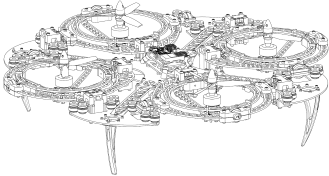
\includegraphics[width=0.93\textwidth]{figs/iso-design}
\caption{Isometric view of the prototype design}
\label{fig:iso-design}
\end{figure}
The final prototype (Fig:\ref{fig:iso-design}) went through a series of different design iterations, aimed at optimizing engineering time spent on construction and reducing the associated component costs. Significant consideration for the design process was the net weight whose upper limit is inherently limited by the thrust produced from lift motors. Some of the more important design factors, like inertial matrices and associated masses (Sec:\ref{sec:proto.inertia}), are discussed here in order to give context for the dynamics derived later in Ch:\ref{ch:dynamics}. The reference frame orientations (which those dynamics are developed with respect to) are detailed here. A brief overview of the electrical systems layout is then given with the components associated and their electrical characteristics included. Finally the actuator suite's functionality and transfer characteristics are quantified. A review of the physical prototype realized and control loop(s) implemented is detailed in Ch:\ref{ch:flight}~along with actual flight test results.
%====================================================
\subsection{Actuation Functionality}
\label{subsec:proto.design.actuation}
%====================================================
The most important component of the design is the manner of articulation for each concentric gimbal ring which forms the four motor module structures. The control objective is to produce a thrust vectoring actuation set for a quadrotor's control plant. The outcome was a module which independently redirects the thrust generated by the lift propellers (Fig:\ref{fig:motor-assembly}). Within each module are servos affixed onto sequential support rings to pitch and roll the substructure's axes. The gyroscope-like frame that surrounds each motor/propeller pair accommodates that relative movement. Aligned with each servo is a coaxial support bearing. The bearing and actuator servos have a mass disparity which results in an eccentric center of mass, producing a net gravitational torque arm. Unfortunately, due to weight constraints, counter balance measures cannot be introduced. Consequences from the center of mass variations must be either compensated for (\emph{plant dependent solution}) or exploited in the dynamics (\emph{additional non-linear actuator plants}). The precise effects are quantified numerically later in Sec:\ref{sec:proto.inertia}.
\par
\begin{figure}[hbtp]
\begin{subfigure}{.49\textwidth}
\centering
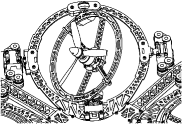
\includegraphics[width=\textwidth]{figs/motor-assembly}
\caption{Motor module assembly}
\label{fig:motor-assembly}
\end{subfigure}
\begin{subfigure}{.49\textwidth}
\centering
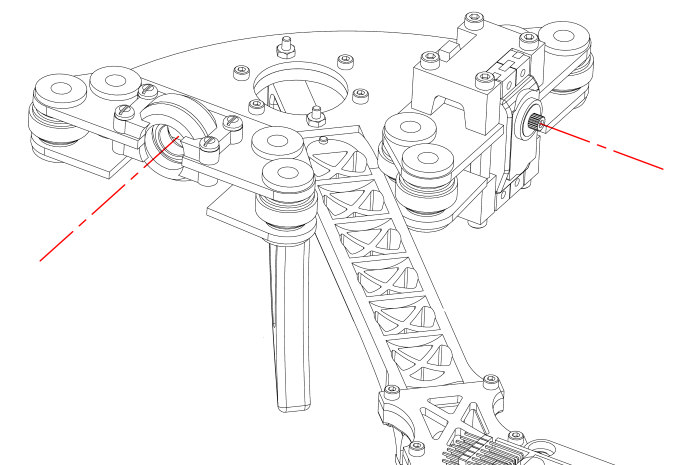
\includegraphics[width=\textwidth]{figs/motor-support}
\caption{Motor frame damping support assemblies}
\label{fig:motor_support}
\end{subfigure}
\caption{Tilting rotor design}
\end{figure}
Each motor module is positioned such that its produced thrust vector coincides with the intersection of its two rotational axes (Fig:\ref{fig:motor-assembly}). As a result there is only a perpendicular displacement, $L_{arm}=195.16~\text{mm}$, co-planar to the body frames X-Y-Z origin $\vec{\mathbf{O}}_b$ (see subsequent Fig:\ref{fig:motor-frame}). That length directly affects the differential torque plant; $\vec{\tau}_{diff}=\sum\vec{L}_i\times\vec{T}_i$. An eccentric thrust vector line would make the torque arm displacement a non-orthogonal vector. The center of gravity for each module is time varying and depends on its two servo rotational positions. It is more prudent to ensure intersection of the thrust vector with the rotational center than to balance the masses undergoing rotation. A thrust varying torque is harder to approximate and hence compensate for than a gravitational torque, given the complexity of modeling a propeller's aerodynamic thrust (Sec:\ref{subsec:dynamics.aero.bem}).
\par
The primary body structure is similar to a traditional quadcopter '+' configuration with adjacent propellers spinning in opposite directions. Each motor module's rotational assembly is suspended by silicone damping balls (Fig:\ref{fig:motor_support}). A smaller damping assembly in the center of the frame houses all the electronics and power distribution circuitry. All the mounting brackets affixing the motor module rings are 3D printed from CAD models using an Ultimaker V2+\cite{ultimaker}. A complete bill of materials for all parts used, including working drawings for each 3D printed bracket and the laser cut frame(s), is presented in Appendix:\ref{app:bom}.
\par
\begin{figure}[hbtp]
\centering
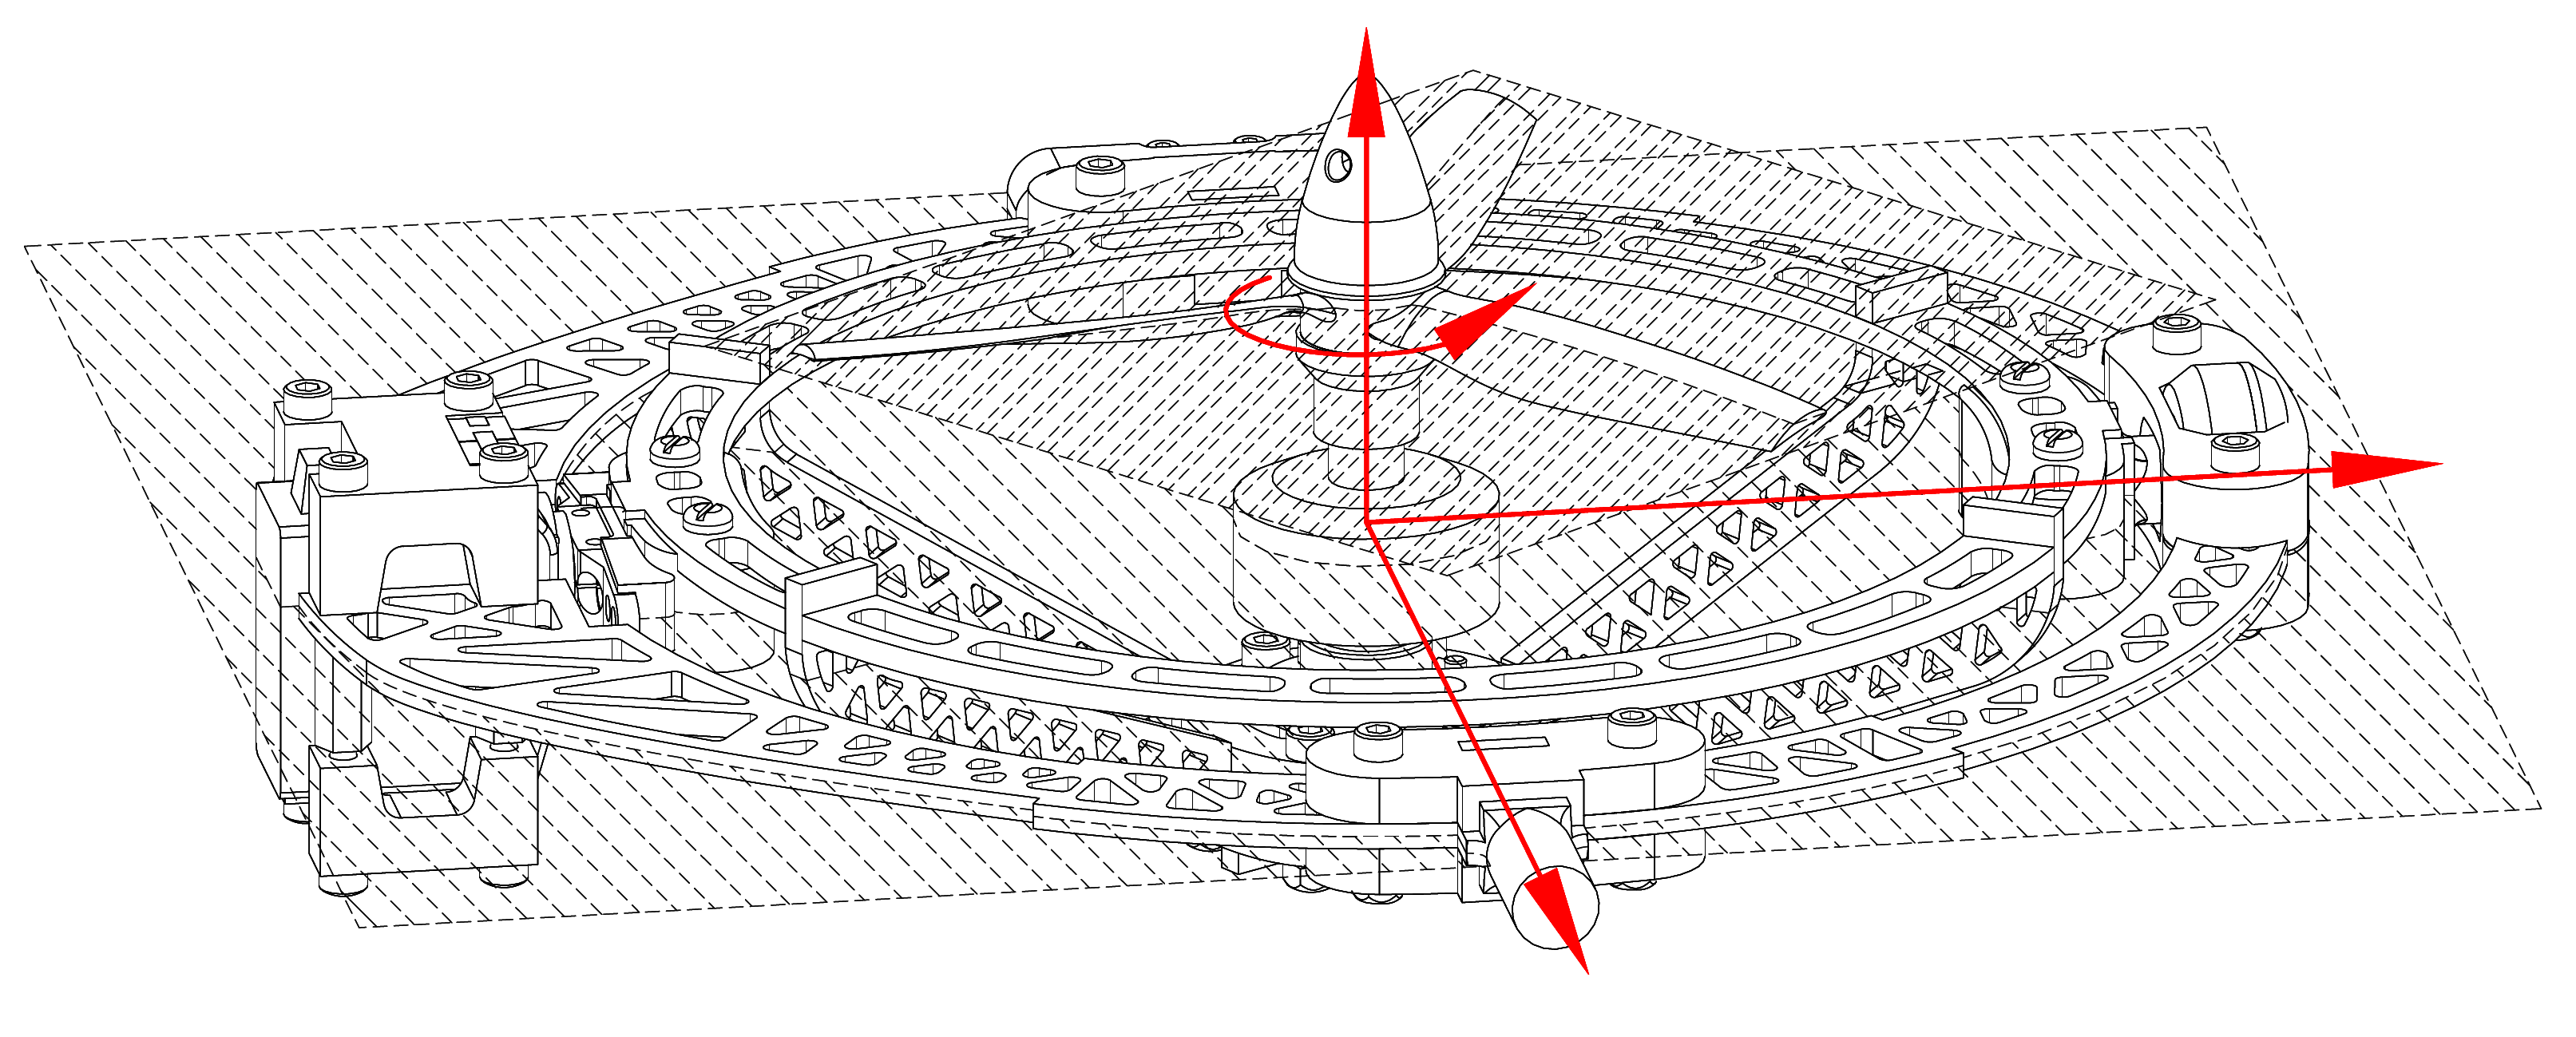
\includegraphics[width=0.85\textwidth]{figs/motor-prop}
\vspace{-10pt}
\caption{Difference between propeller and motor planes}
\label{fig:motor_prop}
\vspace{-15pt}
\end{figure}
The propeller's rotational plane is not aligned exactly with the plane made by the $\hat{X}_{M_i}$ and $\hat{Y}_{M_i}$ rotational servo axes (Fig:\ref{fig:motor_prop}). The offset is approximately $23.4~\text{mm}$ and must be considered when evaluating pitch/roll inertial and gyroscopic torque responses later in Sec:\ref{subsec:dynamics.nonlinearities.gyrotorques}. The propellers are 6 inch ($6 \times 4.5$) 3-Blade plastic Gemfam propellers, powered by Cobra CM2208-2000KV Brushless DC motors (Fig:\ref{fig:bldc-motor}). The thrust produced as a function of angular velocity (in RPS) for the propellers is derived in Sec:\ref{subsec:dynamics.aero.bem}. 
\newpage
The BLDC motors are controlled with LDPower 20A ESC modules with an in-line OrangeRx RPM Sensor. The ESCs were reflashed with BLHeli\cite{BLHeli} firmware. The default firmware on the speed controllers had an unsatisfactory exponential approaching (not linear) input speed curve, in contrast with the linear (unloaded) speed curve in Fig:\ref{fig:rpm-sensor}. The net transfer functions for both ESC modules and the servos are detailed later in Sec:\ref{subsec:proto.design.transfer}. Power for the quadrotor is supplied from a power tether (not from a battery bank). Tethered power will ensure consistent flight time and reduce the concern of payload restriction on the available lift actuation. Power lines to both the BLDC motors and servos are supplied through conventional wiring, however an ideal and more flexible design would see slip-rings for each module's power supply. 
\begin{figure}[htbp]
\centering
\begin{subfigure}{0.49\textwidth}
\centering
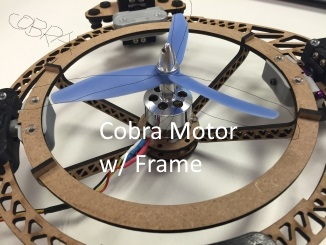
\includegraphics[width=0.9\textwidth]{figs/motor-bldc}
\caption{Cobra CM2208-2000KV BLDC motor module}
\label{fig:bldc-motor}
\end{subfigure}
\begin{subfigure}{0.49\textwidth}
\centering
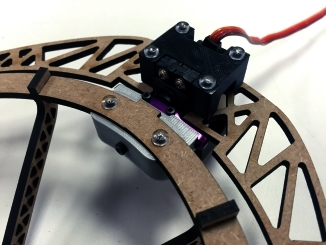
\includegraphics[width=0.9\textwidth]{figs/motor-servo}
\caption{Corona DS-339MG servo bracket}
\label{fig:motor-servo}
\end{subfigure}
\vspace{-5pt}
\caption{Motor module assembly}
\vspace{-15pt}
\end{figure}
\par
Metal gear Corona DS-339MG digital servos are used for the two axes of rotation (Fig:\ref{fig:motor-servo}). Each servo has a rotational range of $\approx\pi$, positioned such that a $\text{zero}^{\text{th}}$ offset aligns the motor modules, adjacent to the body frame, and has a $\pm\pi/2$ rotational range. A digital servo updates at 330 Hz, faster than a 50 Hz analogue servo equivalent (Fig:\ref{fig:servo-timing}). This means the otherwise $20~\text{ms}$ zero-order "analogue" sampling effect is a less significant $3.30~text{ms}$ zero-order holding time. Both the $\hat{X}_{M_i}$ and $\hat{Y}_{M_i}$ axis servos will be rotating a large loading mass and as such their \emph{open loop} plant dynamics are determined empirically in Sec:\ref{subsec:proto.design.transfer}.
\begin{figure}
\centering
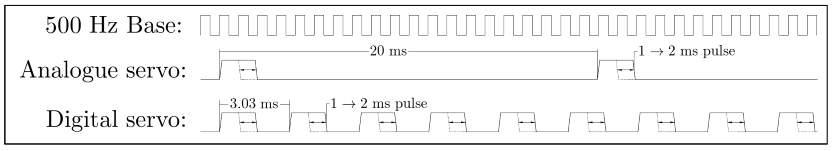
\includegraphics[width=0.75\textwidth]{figs/servo-timing}
\caption{Digital and analogue servo timing}
\label{fig:servo-timing}
\vspace{-20pt}
\end{figure}
%====================================================
\section{Reference Frames Used}
\label{sec:proto.conventions}
Attitude conventions used for deriving the system's dynamics, in Chapter:\ref{ch:dynamics},~are first discussed here. Often these aspects are assumed to be obvious enough that they are omitted. It is important to clearly and unambiguously define a standard set of framing conventions to avoid uncertainty later. Rotation matrices are included but the focus is on the \emph{contrast} between rotation and transformation operations. Both \cite{spacecraftattitutdequaternions} and \cite{rigidbodylecture} provide an in-depth and thorough explanation of rotation matrices and direct cosine matrix attitude representation, if such concepts are unfamiliar to the reader. Quaternions are introduced to replace rotation matrix notation for the dynamics in Sec:\ref{subsec:dynamics.rigidbody.quaternion}.
%====================================================
\subsection{Reference Frames Convention}
\label{subsec:proto.conventions.frames}
%====================================================
\begin{figure}[htbp]
\centering
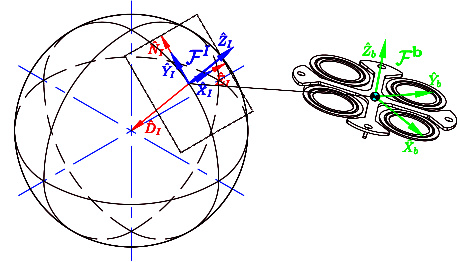
\includegraphics[width=0.8\textwidth]{figs/reference-frame}
\caption{Inertial and body reference frames}
\label{fig:ref_frame}
\end{figure}
NASA aerospace frames are used for principle Cartesian inertial and body coordinate representation (Fig:\ref{fig:ref_frame}). The inertial frame,~$\mathcal{F}^I$, is aligned such that the $\hat{Y}_I$ axis is in the $\hat{N}$orth direction, $\hat{X}_I$ is in the $\hat{E}$ast direction and $-\hat{Z}_I$ is  in the $\hat{D}$ownward direction. In Euler orbital sequences the $\hat{Z}$ direction would be toward the Earth's center, sometimes referred to as the N\^{E}D convention which differs from the NASA frames used here. The body frame, $\mathcal{F}^b$, then has both $\hat{X}_b$ and $\hat{Y}_b$ aligned obliquely between two perpendicular arms of the quadrotor's body and the $\hat{Z}_b$ axis in the body's normal upward direction (illustrated in Fig:\ref{fig:body-frame}). The body frame's axes and center of motion relative to the prototype design's center of mass is related as detailed next in Sec:\ref{subsec:proto.conventions.motoraxis}. Frame superscripts $I$ and $b$ represent inertial and body frames respectively whilst vector subscripts imply the reference frame in which the vector's coordinates exists or taken relative to. 
\begin{equation}
\vec{v}_I=R_b^I(\eta)\vec{v}_b~~~~~~\vec{v}_b\in\mathcal{F}^b,~\vec{v}_I\in\mathcal{F}^I
\end{equation}
Relative angular displacement between two frames is commonly measured by the three angle Euler set. The Euler angle set $\vec{\eta}=[\phi ~\theta ~\psi]^T$ represents pitch $\phi$, roll $\theta$ and yaw $\psi$ rotations about the $\hat{X}$,$\hat{Y}$ and $\hat{Z}$ axes respectively. Depending on how the rotation sequence is formulated, those angles can be used to construct rotation matrices which give relation to vectors or can transform coordinates. The general rotation equation to \emph{rotate} some vector $\vec{v}$ about a normalized unit axis $\hat{u}$ through a rotation angle $\theta$ is given by the formula, proven in \cite{quaddynamics}:
\begin{equation}\label{eq:genrotationmatrix}
\vec{v}~'=\big(1-cos(\theta)\big)\big(\vec{v}\cdot \hat{u}\big)\hat{u}+cos(\theta)\vec{v}+sin(\theta)\big(\hat{u}\times\vec{v}\big)
\end{equation}
In Eq:\ref{eq:genrotationmatrix}, when $\hat{u}$ is in the direction of either $\hat{X}$,$\hat{Y}$ or $\hat{Z}$ axes, the equation can be simplified to produce the three fundamental rotation matrices; $R_x(\phi)$, $R_y(\theta)$ and $R_z(\psi)$. The notation for a rotation matrix operation is multiplication of the matrix $R_{n}(\theta)$, applying a left-handed \emph{rotation} operator about some axis $\hat{n}$ by $\theta$. The resultant vector of a rotation operation still exists in the same reference frame. An $\hat{X}$ axis rotation by $\phi$ of some vector $\vec{v}$ is given by;
\begin{subequations} \label{eq:rotationoperator}
\begin{equation}\label{eq:rotationoperator.a}
\vec{v}^{\hspace{1pt}}\text{}'R_{x}(\phi)\vec{v}~~~~~\vec{v}^{\hspace{2pt}}\text{}',\vec{v}\in\mathcal{F}^1
\end{equation}
\end{subequations}
\emph{\color{Gray} No subscripts are used in Eq: \ref{eq:rotationoperator} to indicate reference frame ownership because all vectors are in the same frame}
\par
A vector \emph{transformation} changes the resultant vector's reference frame. The transformation is then a rotation by an angle of the \emph{difference} between the resulting and principle reference frames. A transformation from frame $\mathcal{F}^1$ to $\mathcal{F}^2$, differing by an angle of $\phi$ about the $\hat{X}$ axis is then a negative rotation operation:
\begin{subequations}\label{eq:transformationoperator}
\begin{equation}\label{eq:transformationoperator.a}
\vec{v}_2=R_x(-\phi)\vec{v}_1
\end{equation}
\vspace{-15pt}
\begin{equation}\label{eq:transformationoperator.b}
\vec{v}_2\in\mathcal{F}^2~\text{and}~\vec{v}_1\in\mathcal{F}^1
\end{equation}
\end{subequations}
The distinction between Eq:\ref{eq:rotationoperator} and Eq:\ref{eq:transformationoperator} is the directional sense of the angular operand $\phi$, and hence the effect it has on the argument vector. The transformation or rotation of a vector from $\mathcal{F}^I$ to $\mathcal{F}^b$ is the product of three sequential operations about each axis. Each subsequent rotation is applied relative to a new intermediate frame; hence each Euler angle is taken relative to a specific intermediate frame and not a global one. The order of those axial rotation operations does affect the Euler set. Any consequences of that chosen order is something discussed in-depth in \cite{rotationsequences}. In this dissertation the Z-Y-X or yaw, pitch, roll rotation sequence is used. A rotation of the vector $\vec{v}$ from the inertial to the body frame, $\mathcal{F}^I\rightarrow\mathcal{F}^b$, is then applied by sequential yaw, $\psi$, pitch, $\theta$, and roll $\phi$ operations:
\\
\begin{subequations}\label{eq:inertialbodyrotation}
\begin{equation}\label{eq:inertialbodyrotation.a}
R_{I}^{b}(\phi,\theta,\psi)\triangleq R_z(\psi)R_y(\theta)R_x(\phi)
\end{equation}
\vspace{-10pt}
\begin{equation}\label{eq:inertialbodyrotation.b}
\vec{v}^{\hspace{1pt}}\text{}'=R_I^b(\phi,\theta,\psi)\vec{v}
\end{equation}
\vspace{-10pt}
\begin{equation}\label{eq:inertialbodyrotation.c}
\rightarrow\vec{v}^{\hspace{1pt}}\text{}'=R_z(\psi)R_y(\theta)R_x(\phi)\vec{v}
\end{equation}
\end{subequations}
It is important to note that in Eq:\ref{eq:inertialbodyrotation} both operand and output vectors are \emph{both} in the inertial frame, $\vec{v}^{\hspace{2pt}}\text{}'~,\vec{v}\in\mathcal{F}^I$. A \emph{transformation} of a vector from the inertial to the body frame is the negative counterpart of Eq:\ref{eq:inertialbodyrotation}, a distinction that is not always explicitly stated.
\begin{subequations}\label{eq:inertialbodytransformation}
\begin{equation}\label{eq:inertialbodytransformation.a}
\vec{v}_b=R_I^b(-\phi,-\theta,-\psi)\vec{v}_I
\end{equation}
\vspace{-15pt}
\begin{equation}\label{eq:inertialbodytransformation.b}
\vec{v}_b\in\mathcal{F}^b~\text{and}~~\vec{v}_I\in\mathcal{F}^I
\end{equation}
\vspace{-12pt}
\begin{equation}\label{eq:inertialbodytransformation.c}
\rightarrow \vec{v}_b=R_z(-\psi)R_y(-\theta)R_x(-\phi)\vec{v}_I
\end{equation}
\vspace{-12pt}
\begin{equation}\label{eq:inertialbodytransformation.d}
=R_x(\phi)R_y(\theta)R_z(\psi)\vec{v}_I=R_{b}^{I}\vec{v}_I
\end{equation}
\vspace{-10pt}
\begin{equation}\label{eq:inertialbodytransformation.e}
R_I^b=\big(R_b^I\big)^{-1}=\big(R_b^I\big)^T
\end{equation}
\end{subequations}
The relationship in Eq:\ref{eq:inertialbodytransformation.e} is an inversion property (\emph{transpose}) of the rotation matrix. A rotation matrix's inverse can be used interchangeably with its negative counterpart to maintain a positive sense of the argument angle. To ensure clarity throughout this dissertation's mathematics, a negative angular sense implies a \emph{transformation} to a different reference frame. Where applicable, the order of rotation will indicate the sequence direction whilst the angular sign differentiates the rotation or transformation operations.
\par
The body frame's angular velocity is taken relative to the inertial frame, represented by $\vec{\omega}_{b/I}$ mostly just simplified to $\vec{\omega}_b$. Seeing that each Euler angle is measured with respect to an intermediary frame, a distinction must then be made between $d\vec{\eta}/dt$ and $\vec{\omega}_b$. All three Euler angles need to be transformed to one common frame to define the relationship between Euler and angular rates. 
\par
Exploiting vehicle frames 1 \& 2, or rather $\mathcal{F}^{v1}$ \& $\mathcal{F}^{v2}$, as intermediary frames to respectively describe frames after $R_x(\phi)$ and $R_y(\theta)$ operations. The angular velocity $\vec{\omega}_b$ is the time derivative of Euler angles in the body frame:
\begin{subequations}
\begin{equation}\label{eq:angular-rates.a}
\vec{\omega}_b=\begin{bmatrix}
p & q & r
\end{bmatrix}^T
=
\frac{d}{dt_b}\vec{\eta}=\frac{d}{dt}\vec{\eta}_b~~~~\in\mathcal{F}^b
\end{equation}
\begin{equation}
\vec{\eta}_b = R_{v_2}^b(\phi)\begin{bmatrix}
\phi\\
0\\
0
\end{bmatrix}
+R_{v_2}^b(\phi)R_{v_1}^{v_2}(\theta)\begin{bmatrix}
0\\
\theta\\
0
\end{bmatrix}
+R_{v_2}^b(\phi)R_{v_1}^{v_2}(\theta)R_I^{v_1}(\psi)\begin{bmatrix}
0\\
0\\
\psi
\end{bmatrix}~~~~\in\mathcal{F}^b
\end{equation}
\begin{equation}
\therefore\dot{\vec{\eta}}_b=\frac{d\phi}{dt}R_{v2}^b(\phi)\begin{bmatrix}
\phi\\
0\\
0\\
\end{bmatrix}
+
\frac{d\theta}{dt}R_{v2}^{b}(\phi)R_{v1}^{v2}(\theta)\begin{bmatrix}
0\\
\theta\\
0
\end{bmatrix}
+
\frac{d\psi}{dt}R_{v2}^{b}(\phi)R_{v1}^{v2}(\theta)R_{I}^{v1}(\psi)\begin{bmatrix}
0\\
0\\
\psi
\end{bmatrix}
\end{equation}
\emph{\color{Gray}The vehicle frames in Eq:\ref{eq:angular-rates.a} and the subsequent rotations between each frame don't necessarily have to be in that order. The equation could change depending on what rotation sequence was used, here Z-Y-Z rotation sequences were used\ldots}
\par
Which then simplifies to the formal relationship between two rotating frames, with $\vec{\omega}_b=[p~q~r]^T$ in $rad.s^{-1}$:
\begin{equation}\label{eq:angular-rates.b}
\begin{bmatrix}
p\\
q\\
r\\
\end{bmatrix}
=
\begin{bmatrix}
1 & 0 & -sin(\theta)\\
0 & cos(\phi) & sin(\phi)cos(\theta)\\
0 & -sin(\theta) & cos(\phi)sin(\theta)\\
\end{bmatrix}
\begin{bmatrix}
\dot{\phi}\\
\dot{\theta}\\
\dot{\psi}\\
\end{bmatrix}
\end{equation}
\begin{equation}\label{eq:angular-rates.c}
\Rightarrow\vec{\omega}_b=\Psi(\eta)\dot{\vec{\eta}}~~~~\in\mathcal{F}^b
\end{equation}
\begin{equation}\label{eq:angular-rates.d}
\Psi(\eta)=
\begin{bmatrix}
1 & 0 & -sin(\theta)\\
0 & cos(\phi) & sin(\phi)cos(\theta)\\
0 & -sin(\theta) & cos(\phi)sin(\theta)\\
\end{bmatrix}
\end{equation}
\begin{equation}\label{eq:angular-rates.e}
\Rightarrow\dot{\vec{\eta}}=\Psi^{-1}(\eta)\vec{\omega}_b=\Phi(\eta)\vec{\omega}_b~~~~\in\mathcal{F}^{v1,v2,I}
\end{equation}
\begin{equation}\label{eq:angular-rates.f}
\Phi(\eta)=\begin{bmatrix}
1 & sin(\phi)tan(\theta) & cos(\phi)tan(\theta)\\
0 & cos(\phi) & -sin(\phi)\\
0 & sin(\phi)sec(\theta) & cos(\phi)sec(\theta)\\
\end{bmatrix}
\end{equation}
\end{subequations}
\par
The termed \emph{Euler} matrix, $\Phi(\eta)$, contains a well known and problematic singularity at $\theta=\pm\pi/2$; because $sec(\theta)\rightarrow\infty$ as $\theta\rightarrow\pi/2$, as such $\Psi(\eta)$ looses rank. The mathematical manifestation of the rotation matrix singularity and its practical implications are further explored later in Sec:\ref{subsec:dynamics.rigidbody.singularity}. The singularity is present in the middle roll rotation angle, $\theta$, which is a direct consequence of the chosen Z-Y-X rotation sequence adopted. 
\par
Each Euler angle can potentially suffer its own singularity depending on how the rotations are ordered. Indeed quaternions are used for kinematics later in lieu of Euler angles in later dynamics (Sec:\ref{subsec:dynamics.rigidbody.quaternion}). Euler angular attitude representations are, however, easily understood and well suited to the conventional definitions made in this Chapter.
\par
Quaternion operations are similarly constructed in the Z-Y-X order. Quaternion operations are additive and not commutative. The sequenced quaternion order will produce the same resultant frame rotation however the quaternion and its rotation path will differ. For a quaternion $Q_b$ representing the body's attitude:
\begin{subequations}
\begin{equation}\label{eq:quaternion-rotation-equivalence}
\vec{v}_b=R_I^b\vec{v}_I\underset{Q}{\iff} Q_b \otimes \begin{bmatrix}
0\\
\vec{v}_I
\end{bmatrix} \otimes Q_b^*
\end{equation}
\begin{equation}
Q_b \triangleq Q_z Q_y Q_x~~\text{and it's inverse}~~Q_b^* \triangleq Q_x^* Q_y^* Q_z^*
\end{equation}
\end{subequations}
With $\otimes$ being the Hamilton product or quaternion multiplication operator, the Hamilton product is used again for inertial tensor transformations later in Sec:\ref{sec:proto.inertia}. Each quaternion, $Q_{\hat{i}}$, is always the unit quaternion about that $\hat{i}^{th}$ axis. For the body quaternion, $Q_b$, it is unit quaternion rotation about the body's singular Euler axis\cite{rotationsequences}. It is important to note that a quaternion rotation operates on an argument vector with a zero quaternion scalar component. So then for some vector $\vec{v}$, the quaternion rotation operation in Eq:\ref{eq:quaternion-rotation-equivalence} is equivalent to;
\begin{subequations}
\begin{equation}\label{eq:quaternion-operator.a}
Q_{\vec{v}^{\hspace{1pt}}\text{}'}=Q \otimes (Q_{\vec{v}}) \otimes Q^*
\end{equation}
\vspace{-10pt}
\begin{equation}\label{eq:quaternion-operator.b}
\text{Where}~Q_{\vec{v}}=\begin{bmatrix}
0\\
\vec{v}\hspace{2pt}\\
\end{bmatrix},~Q_{\vec{v}^{\hspace{1pt}}\text{}'}=\begin{bmatrix}
0\\
\vec{v}^{\hspace{1pt}}\text{}'\\
\end{bmatrix}
\end{equation}
\end{subequations}
The quaternion representation in Eq:\ref{eq:quaternion-operator.b} ensures that the operation is entirely in $\mathbb{R}^4$ space. However it is typically omitted, despite $\mathbb{R}^4$ being implied and as such, Eq:\ref{eq:quaternion-operator.a} is then simply:
\begin{equation}
\vec{v}^{\hspace{1pt}}\text{}'=Q \otimes (\vec{v}\hspace{2pt}) \otimes Q^*
\end{equation}
Quaternion dynamics, and the quaternion operator, are later expanded upon to replace the use of Euler angles and rotation matrices as a convention for attitude representation later in Chapter:\ref{ch:dynamics}. Quaternion dynamics are widely regarded as the better choice for aerospace attitude representation due to their dual coverage and globally non-singular nature.
%====================================================
\subsection{Motor Axis Layout}
\label{subsec:proto.conventions.motoraxis}
%====================================================
Fundamentally the whole structure consists of multiple rigidly connected bodies with only relative rotations between each body permitted by its joints, illustrated previously in the design description in Sec:\ref{sec:proto.design}. Those rigid bodies are categorized into four inter-connected motor modules, $\mathbb{M}_{1\rightarrow 4}$, and a single body structure, $\mathbb{B}$ (\emph{frame} structure, not reference frame). Each module consists of two sequential gimbal rings, each with one degree of relative rotation between itself and the subsequent ring. There needs to be distinct nomenclature used for describing these motor modules such that the dynamic derivations later are clear and logical despite the complicated multibody system. 
\begin{figure}[htbp]
\centering
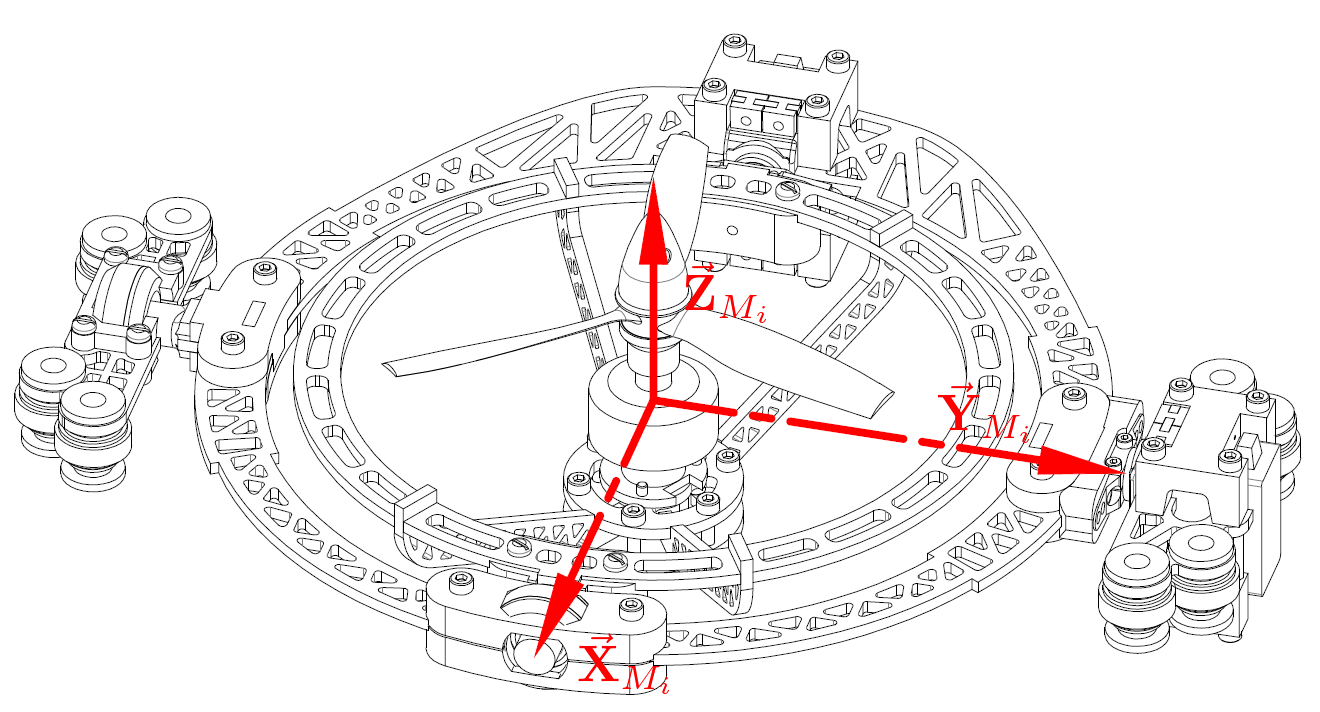
\includegraphics[width=0.85\textwidth]{figs/motor-axes}
\caption{Aligned motor frame axes}
\label{fig:motor-axes}
\vspace{-10pt}
\end{figure}
\par
Every propeller/motor pair is actuated by two servos. The $i^{th}$ propeller for motor module $\mathbb{M}_i$ in frame $\mathcal{F}^{M_i}$, directly driven by the motor's rotor, has a rotational speed $\Omega_i~\text{[RPS]}$ about the $\hat{Z}_{M_i}$ stator axis. Two servos are aligned \emph{at rest} with the motor's $\hat{X}_{M_i}$ and $\hat{Y}_{M_i}$ axes to pitch and roll the propeller away from its principle frame. Each motor has its own reference frame, $\mathcal{F}^{M_i}$, aligned as shown in Fig:\ref{fig:motor-axes} and highlighted with the rotational rings in Fig:\ref{fig:motor-frame}.
\par
\begin{minipage}{\textwidth}
\begin{wrapfigure}{r}{0.55\textwidth}
\centering
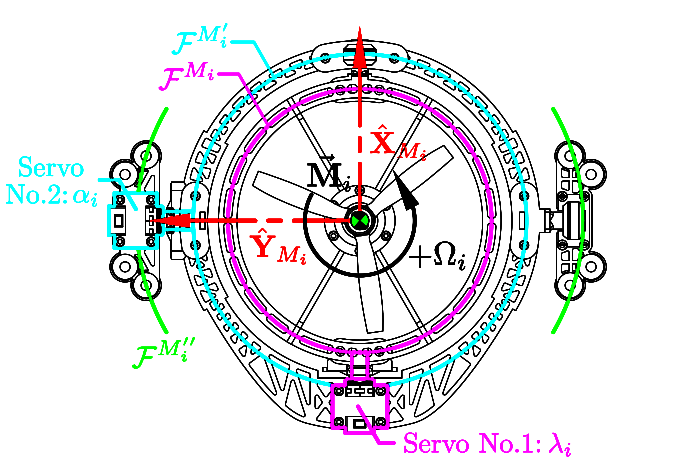
\includegraphics[width=0.55\textwidth]{figs/motor-frame}
\caption{Intermediate motor frames}
\label{fig:motor-frame}
\end{wrapfigure}
\par
Motor frames, numbered $1\rightarrow 4$, transform to the body frame first by an angle of $\lambda_i$ about the $\hat{X}_{M_i}$ axis. Then by $\alpha_i$ about the $\hat{Y}_{M_i'}$ axis in an intermediate $M_i'$ frame. The first servo actuates $\lambda_i$, rotating $\mathcal{F}^{M_i}$ to an intermediate $\mathcal{F}^{M_i'}$ frame. Secondly, the next servo actuates $\alpha_i$ to produce a second intermediate frame $M_i''$. That second servo is affixed in the $M_i''$ frame. Lastly there's a relative orthogonal rotation about $\hat{Z}_{M_i''}$ between $\mathcal{F}^b$ and $\mathcal{F}^{M_i''}$. Each module's actuation state is fully described by $[\Omega_{i}~\lambda_{i}~\alpha_{i}]^{T}$ for $i\in [1:4]$. The four motor modules are aligned relative to the body's XYZ axes as shown in Fig:\ref{fig:body-frame}. Modules 1 and 3 have their X-axes in the positive and negative $\hat{X}_b$ directions of the body frame respectively. Similarly Modules 2 and 4 have their X-axes in the positive and negative $\hat{Y}_b$ directions of the body frame.
\end{minipage}
\par
\begin{figure}[htbp]
\centering
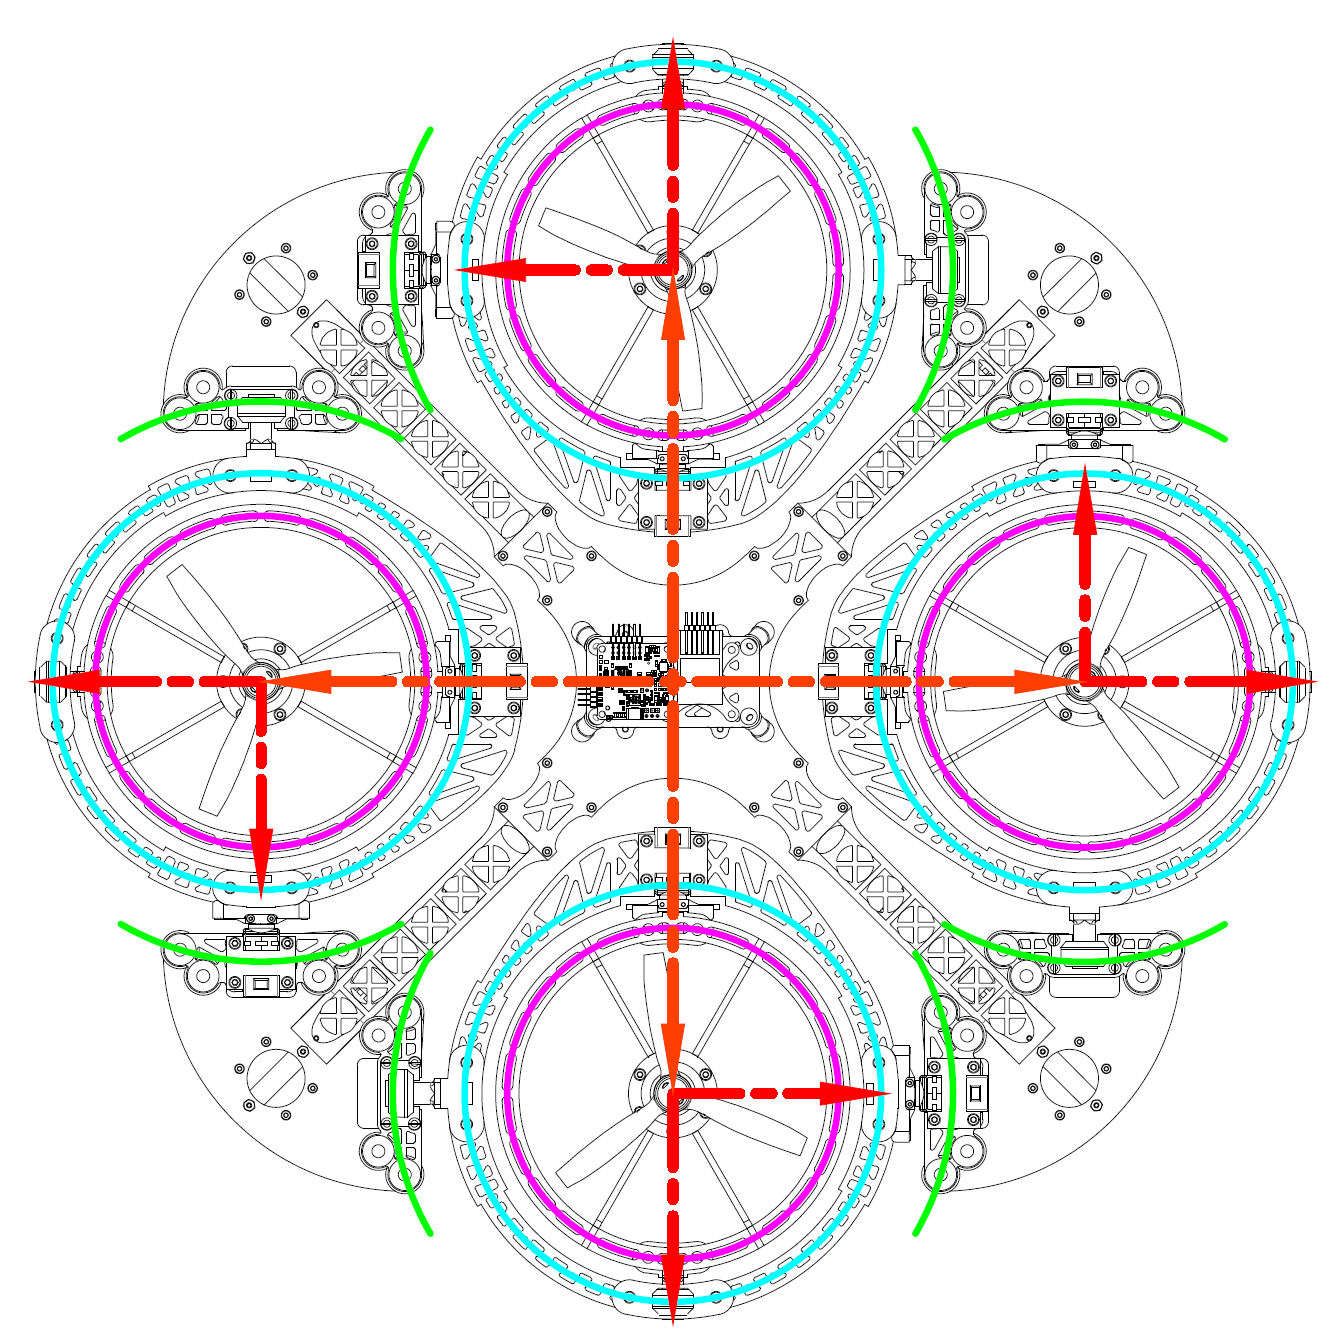
\includegraphics[width=0.88\textwidth]{figs/body-frame}
\caption{Body frame axes layout}
\vspace{-15pt}
\label{fig:body-frame}
\end{figure}
\par
\emph{\color{Gray}Not shown in Fig:\ref{fig:body-frame} is the relative $\hat{Z}$ axis position with respect to the structure. The $\hat{Z}$ height of the body's motion centroid is such that its origin is co-planar with the four motor modules rotational centers. The center of motion is \underline{not} the center of mass, an aspect which is discussed next in Sec:\ref{sec:proto.inertia}.}
\par
Motor modules 1 \& 3 have clockwise (\emph{positive}) rotating propellers denoted by $\Omega_{[1,3]}^{+}$. Conversely modules 2 \& 4 have counter-clockwise (\emph{negative}) rotations denoted by $\Omega_{[2,4]}^{-}$. Vector transformations from each of the four motor frames to the body frame are characterized as:
\begin{subequations}
\begin{equation}\label{eq:motor-module-rotation.a}
\vec{v}_b=R_z(-\sigma_i)R_y(-\alpha_i)R_x(-\lambda_i)\vec{v}_{M_i}~~\text{for}~~\sigma_i\in\frac{1}{2}[0,~\pi,~2\pi,~3\pi]
\end{equation}
The orthogonal $\sigma_i$ rotations about $\hat{Z}_{M_i''}$ are constant and determined by the motor module number. Their associated rotation matrices $R_z(\sigma_i)$ are given by:
\begin{equation}\label{eq:motor-module-rotation.b}
R_z=\begin{bmatrix}
1 & 0 & 0\\
0 & 1 & 0\\
0 & 0 & 1
\end{bmatrix}, \begin{bmatrix}
0 & -1 & 0\\
1 & 0 & 0\\
0 & 0 & 1
\end{bmatrix}, \begin{bmatrix}
-1 & 0 & 0\\
0 & -1 & 0\\
0 & 0 & 1
\end{bmatrix}, \begin{bmatrix}
0 & 1 & 0\\
-1 & 0 & 0\\
0 & 0 & 1
\end{bmatrix}~\text{for}~i\in[1,2,3,4]~\text{respectively}
\end{equation}
\label{eq:motor-module-rotation}
\end{subequations}
\\
The entire actuator space, including propeller speed $\Omega_i~\text{[RPS]}$, is then $\in\mathbb{R}^{12}$, or rather $\mathbb{U}\in\mathbb{R}^{12}$, in contrast with $\mathbb{U}\in\mathbb{R}^4$ for a standard quadrotor. The actuator input set $u \in \mathbb{U}$ is then structured as:
\begin{equation}
\underset{\in\mathbb{U}}{u}=\begin{bmatrix}
\Omega_1^+ & \lambda_1 & \alpha_1 & \ldots & \Omega_4^- & \lambda_4 & \alpha_4
\end{bmatrix}^T
\end{equation}
%====================================================
\section{Inertial Matrices \& Masses}
\label{sec:proto.inertia}
%====================================================
\emph{\color{Gray}Although inertias are presented here rounded to either 2 or 0 decimal places, full floating point numbers are used in simulation and prototype software. In some cases when transforming inertias it is more appropriate to use rotation matrices to apply the transformation and not quaternions. Spatial rotation of inertial tensors are ill suited to quaternion parametrization.}
\par
An undesirable side effect of the relative rotations within a non-rigid body are the inertial responses associated with such movements. Given Newton's Second Law of Rotational Motion; each applied rotation is going to produce an equal but opposite reaction onto the principle inducing body. Similarly a gyroscopic cross product from rotational velocities is also present when rotating bodies that have their own relative rotation. Such first and second order effects are often neglected given that the angular rates which they are dependent on are mostly small enough to approximate as zero, $\vec{\omega}_b\approx\vec{0}$. A dynamic set-point (non-zero) attitude tracking plant is, however, going to produce non-zero time varying body angular velocities and accelerations. Unlike a traditionally actuated quadrotor, such effects will need to be compensated for.
\par
The manifestation of those torque responses are derived next in Sec:\ref{subsec:dynamics.nonlinearities.gyrotorques}. Both inertial and gyroscopic effects are dependent on the rotational body's moment of inertia about each respective rotational axis. The magnitude of those inertias are obviously a by-product of the structure's design. The following inertias presented are all calculated from a SolidWorks model with masses to match physical prototype measurements. Each rigidly connected body affected by the same angular velocity is grouped together into inertial matrices. Every motor module then has 3 such assemblies; the propeller/rotor body, the inner ring and middle ring assemblies which are now described and expanded. 
\par
The first rotational body to consider is that of the propeller and rotor assembly (Fig:\ref{fig:inertia-prop}, excluding the motors stator). The "rotor" assembly has a net mass $\text{m}_{\text{rot}}=27~\text{g}$ with a center of mass $\text{C.M}_{\text{rot}}=\begin{bmatrix}0&0&19.5\end{bmatrix}^T~[\text{mm}]$ relative to the entire motor modules center of rotation. It is important to reiterate that the propeller's plane of rotation is $\begin{bmatrix}0&0&23.4\end{bmatrix}^T~[\text{mm}]$ relative to the entire body's center of rotation (Fig:\ref{fig:motor_prop}). At high speeds the propellers inertial contribution is simplified that of a solid disc. 
\par
The entire rotor assembly then has an inertia $J_{rot}$, with principle inertial axes aligned as in Fig:\ref{fig:inertia-prop}:
\begin{equation}
J_{rot}=\begin{bmatrix}
151.71 & 0.00 & 0.00\\
0.00 & 151.66 & 0.00\\
0.00 & 0.00 & 34.07
\end{bmatrix}~~~~[\text{g.cm}^2]
\end{equation}
The net angular velocity of the rotor assembly relative to the body frame is produced by the BLDC motor's own rotational velocity $\Omega_i$ and the servo rates; $\dot{\lambda}_i$ and $\dot{\alpha}_i$. Both servo rates are transformed onto the motor frame $\mathcal{F}^{M_i}$.
\begin{equation}\label{eq:net-angular-rot}
\vec{\omega}_{rot}=\begin{bmatrix}
0\\
0\\
\Omega_i
\end{bmatrix}
+\frac{d\lambda_i}{dt}\big(R_x(\lambda_i)\big)\begin{bmatrix}
\dot{\lambda_i}\\
0\\
0
\end{bmatrix}+\frac{d\alpha_i}{dt}\big(R_y(\alpha_i)R_x(\lambda_i)\big)\begin{bmatrix}
0\\
\dot{\alpha_i}\\
0
\end{bmatrix}~~~~\in\mathcal{F}^{M_i}
\end{equation}
\emph{\color{gray} Eq:\ref{eq:net-angular-rot} is later replaced with a quaternion operator. That equation and the remaining angular velocity equations for each body derived here are therefore not expanded further in their current rotation matrix form(s)\ldots}
\begin{figure}[htbp]
\centering
\begin{subfigure}{0.49\textwidth}
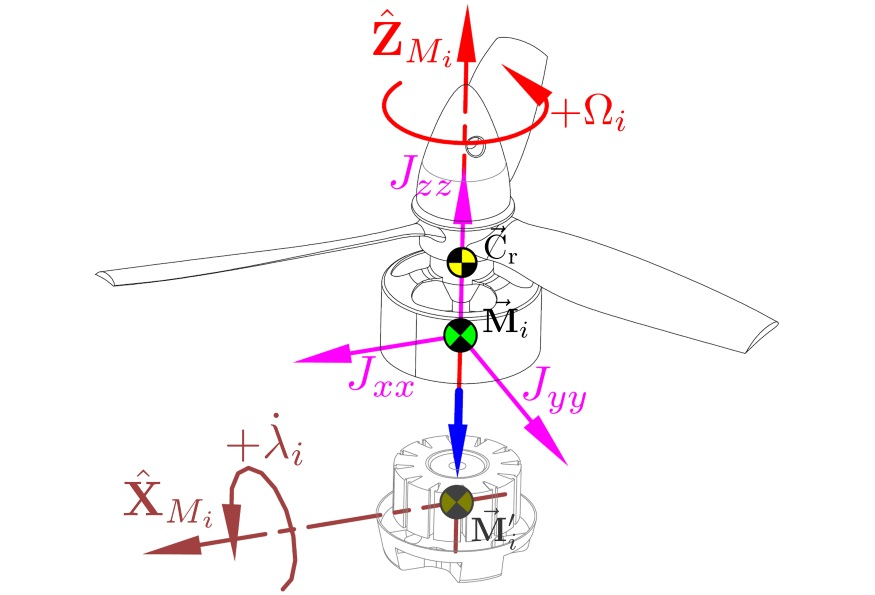
\includegraphics[width=\textwidth]{figs/inertia-prop}
\caption{Rotor assembly rotational structure}
\label{fig:inertia-prop}
\end{subfigure}
\begin{subfigure}{0.49\textwidth}
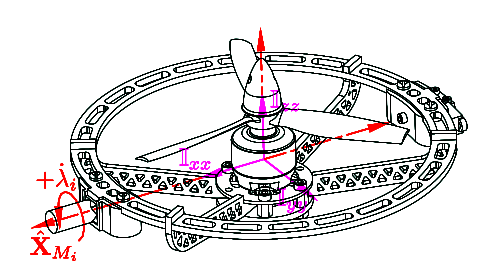
\includegraphics[width=\textwidth]{figs/inertia-inner}
\caption{Inner ring rotational structure}
\label{fig:inertia-inner}
\end{subfigure}
\caption{Inertial measurement references}
\end{figure}
\par
The next assembly, onto which the motor frame $\mathcal{F}^{M_i}$ is attached to, is the inner ring assembly. The inner ring structure is a $92~[\text{g}]$ body, including the rotor assembly in that calculation. The center of mass is positioned $\text{C.M}_{\text{inner}}=\begin{bmatrix}-1.44&0&5.81\end{bmatrix}^T~[\text{mm}]$ relative to the center of rotation $\vec{\mathbf{M}}_i$. The inner ring, being rotated by the $\lambda_i$ servo about the $\hat{X}_{M_i}$ axis, then has an inertial matrix (centered and aligned with axes as in Fig:\ref{fig:inertia-inner}):
\begin{equation} \label{eq:inertia.inner}
J_{inner}=J_{M_i}=\begin{bmatrix}
520.8 & -31.7	& -0.3\\
-31.7 & 1836.3 & 0.00\\
-0.3 & 0.00	& 2050.9\\
\end{bmatrix}~~~~[\text{g.cm}^2]
\end{equation}
The effect of rapidly spinning propellers, relative to the servo rotational velocity, on the inertia in Eq:\ref{eq:inertia.inner} is approximated well by a solid disc. The inner ring's inertial components are then regarded as constant with respect to $\Omega_i$, moreover its center of mass is independent of that propeller's rotation. Given the order of magnitude of the inertia ($\times 10^{-7}$), it is fair to simplify the inner ring's inertial matrix to a diagonal matrix $J_{M_i}\approx diag\begin{pmatrix}521&1836&2051\end{pmatrix}\times10^{-7}~[\text{kg.m}^2]$. The rotational velocity of the inner ring assembly, $\vec{\omega}_{inner}$ or $\vec{\omega}_{M_i}$ for simplicity as it is the velocity of the inner ring frame $\mathcal{F}^{M_i}$, is similar to that of Eq:\ref{eq:net-angular-rot} and occurs in the same frame, without the added rotor rotation of $\Omega_i$:
\begin{equation}\label{eq:net-angular-inner}
\vec{\omega}_{inner}=\vec{\omega}_{M_i/b}=\frac{d\lambda_i}{dt}\big(R_x(\lambda_i)\big)\begin{bmatrix}
\dot{\lambda}_i\\
0\\
0
\end{bmatrix}
+\frac{d\alpha_i}{dt}\big(R_y(\alpha_i)R_x(\lambda_i)\big)\begin{bmatrix}
0\\
\dot{\alpha}_i\\
0
\end{bmatrix}~~~~\in\mathcal{F}^{M_i}
\end{equation}
That first actuating servo for $\lambda_i$ and its coaxial support bearing are both affixed to the intermediate middle ring assembly (Fig:\ref{fig:inertia-middle}). The middle ring assembly, attached to the frame $\mathcal{F}^{M_i'}$, is a $98~[\text{g}]$ body, excluding the inner most ring's contribution, with a center of mass $\text{C.M}_{\text{middle}}=\begin{bmatrix}
-4.70&0.37&-0.36\end{bmatrix}^T~[\text{cm}]$ relative the center of rotation $\vec{\mathbf{M}}_i$.
\par
Together the inner and middle rings form the motor module assembly, with a mass $m_{module}=190~[\text{g}]$. That center of mass for the motor module varies dependent on the inner ring's rotational position $\lambda_i$. The module's center of mass $\text{C.M}_{\text{module}}$ is calculated as follows:
\begin{subequations}
\begin{equation}
\text{C.M}_{\text{inner}}'=R_x(\lambda)\big(\text{C.M}_{\text{inner}}\big)
\end{equation}
\vspace{-10pt}
\begin{equation}
\text{C.M}_{\text{module}}=\frac{m_{middle}\big(\text{C.M}_{\text{middle}}\big)+m_{inner}\big(\text{C.M}_{\text{inner}}'\big)}{m_{middle}+m_{inner}}
\end{equation}\vspace{-4pt}
\begin{equation}
\text{C.M}_{\text{module}}(\lambda)=\frac{98\begin{bmatrix}-4.70 & 0.37 & -0.36\end{bmatrix}^T\times 10^{-7}+R_x92(\lambda)\begin{bmatrix}
-1.44& 0 & 5.81
\end{bmatrix}^T\times 10^{-8}}{190\times 10^{-3}}
\end{equation}
\vspace{-4pt}
\begin{equation}
\text{C.M}_{\text{module}}(0)=	\begin{bmatrix}
-2.49 & 0.19 & 0.12
\end{bmatrix}^T\Big|_{\lambda_i=0}~~~~[\text{cm}]
\end{equation}
\end{subequations}
The motor module assembly is rotated by the $\alpha_i$ servo about its $\hat{Y}_{M_i'}$ axis. The module's compound body inertia, $J_{module}$, is a combination of the middle ring's inertia $J_{middle}$ and the inner ring's inertia $J_{inner}$ rotated by $\lambda_i$ about $\hat{X}_{M_i}$ (aligned as per Fig:\ref{fig:inertia-module}). The latter's contribution is dependant on the \emph{rotation} (not transformation) angle $\lambda_i$ which from the conservation of angular momentum theory, detailed concisely in \cite{rigidbodyinertia}, produces the net inertia $J_{M_i'}$:
\begin{subequations}\label{eq:inertia.middle}
\begin{equation} \label{eq:inertia.middle.a}
\text{With} ~~J_{middle}=\begin{bmatrix}
2905.70 & 0.02 & 390.89\\
0.02 & 8446.41 & 0.01\\
390.89 & 0.01 & 11125.74\\
\end{bmatrix}~~~[g.cm^2]
\end{equation}
\vspace{-5pt}
\begin{equation}\label{eq:inertia.middle.b}
J_{M_i'}=J_{middle}+R_{x}(\lambda_i)\big(J_{inner}\big)R_{x}^{-1}(\lambda_i)
\end{equation}
Because $R_x$ is a full rank square matrix, its inverse $R^{-1}_{x}$ used in Eq:\ref{eq:inertia.middle.b} always exists. The modules inertia can be further divided into constant and variable components\ldots
\begin{equation}\label{eq:inertia.middle.c}
J_{M_i'}(\lambda_i)=J_{const}+J_{M_i}(\lambda_i)
\end{equation}
\vspace{-10pt}
\begin{equation} \label{eq:inertia.middle.d}
\approx\begin{bmatrix}
3427 & 0 & 391\\
0 & 10497 & 0\\
391 & 0 & 12952\\
\end{bmatrix}
+
\begin{bmatrix}
0 & -32{c}_{\lambda} & -32{s}_{\lambda}\\
-32{c}_{\lambda} & -225{c}^2_{\lambda} & 112s_{2\lambda}\\
-32{s}_{\lambda} & 112s_{2\lambda} & 225{c}^2_{\lambda}\\
\end{bmatrix}
\times10^{-7}~~~[kg.m^2]
\end{equation}
\end{subequations}
\begin{figure}[htbp]
\begin{subfigure}{0.49\textwidth}
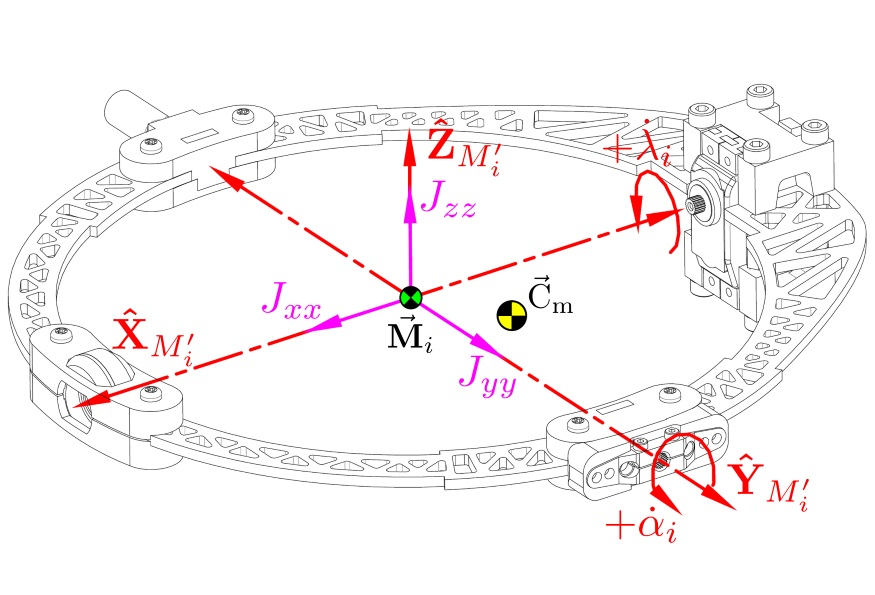
\includegraphics[width=\textwidth]{figs/inertia-middle}
\caption{Middle ring rotational structure}
\label{fig:inertia-middle}
\end{subfigure}
\begin{subfigure}{0.49\textwidth}
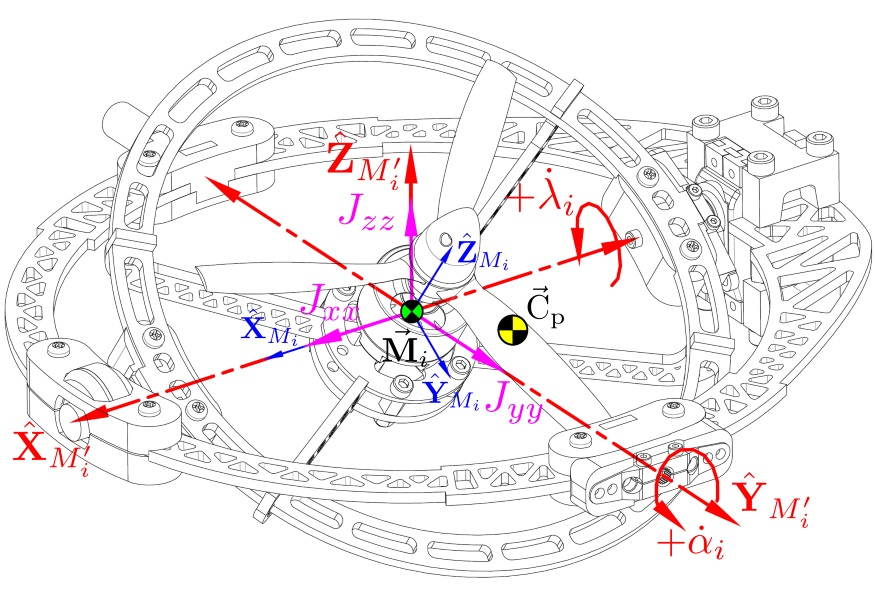
\includegraphics[width=\textwidth]{figs/inertia-module}
\caption{Module assembly rotational structure}
\label{fig:inertia-module}
\end{subfigure}
\caption{Inertial measurement references cont.}
\vspace{-20pt}
\end{figure}
\par
Where $J_{M_i}=J_{inner}$ is the inner ring's inertia from Eq:\ref{eq:inertia.inner}, re-orientated through a rotation $R_x(\lambda_i)$; the convention here is that $s\lambda$ and $c\lambda$ are short handed for $\sin(lambda)$ and $cos(\lambda)$ respectively. The module's net inertia is a combination of an inertia as a function of the rotation angle $\lambda_i$ and a constant inertial component (Eq:\ref{eq:inertia.middle.c}), which together are then simplified to Eq:\ref{eq:inertia.middle.d}. Note that Eq:\ref{eq:inertia.middle.d} is rounded to no decimal places here but in practice the full floating point matrix is used. Finally, the angular velocity experienced by the net motor assembly, $\vec{\omega}_{module}$ in frame $\mathcal{F}^{M_i'}$, is solely as a result of the $\alpha_i$ servo rotation:
\begin{equation}
\vec{\omega}_{module}=\vec{\omega}_{M_i'/b}=\frac{d\alpha_i}{dt}\big(R_y(\alpha_i)\big)\begin{bmatrix}
0\\
\dot{\alpha}_i\\
0
\end{bmatrix}~~~~\in\mathcal{F}^{M_i'}
\end{equation}
\par
Variable inertias dependent on state input variables are one of many non-trivial aspects unique to the multibody design. Control solutions are thus decidedly plant dependent in their formulation. The center of mass for each motor module's compound assembly coincides with neither rotational axes' intersections. As a result the effective center of mass for each module, and the entire structure, is going to be a time varying function each motor module's angular rotational position.
\begin{figure}[hbtp]
\begin{subfigure}{0.49\textwidth}
\centering
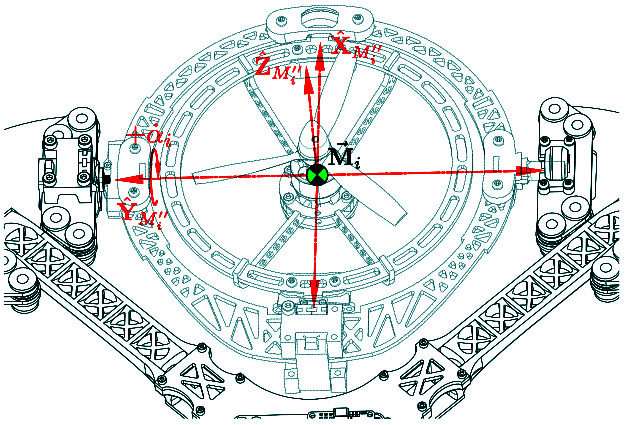
\includegraphics[width=\textwidth]{figs/inertia-damping}
\caption{Damping assembly attached to frame}
\label{fig:inertia-damping}
\end{subfigure}
\begin{subfigure}{0.49\textwidth}
\centering
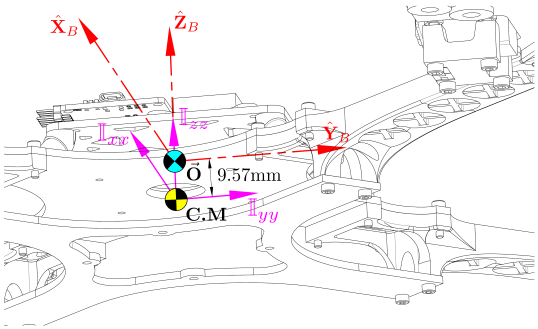
\includegraphics[width=\textwidth]{figs/inertia-center}
\caption{Body structure's center of mass}
\label{fig:inertia-center}
\end{subfigure}
\caption{}
\label{fig:damping-center}
\vspace{-15pt}
\end{figure}
\par
The second servo that rotates $\alpha_i$ adjoins the complete motor module (both the inner and middle ring assemblies) to the body structure. The inertial volume of the second pair of servo and bearing supports contribute then to the body structure's inertia; whose value excludes any of the four motor modules (Fig:\ref{fig:inertia-damping}). Consisting of servo and bearing damping brackets, each "damping" assembly collectively weighs $84g$ and suspends the motor modules from the body frame with a set of silicon damping balls. The body structure's center of mass (without motor modules attached, Fig:\ref{fig:inertia-center}) coincides with the XY directional axes and lies $\Delta Z=-9.52~[\text{mm}]$ below the Body Frame's origin of motion; $\vec{\mathbf{O}}_b\in\mathcal{F}^b$.
\\
\emph{\color{Gray}Note: that body frame origin which all motion is calculated with respect to is co-planar to the motor module's rotational centers, \underline{not} the net center of mass.}
\par
The body's weight, including all four damping assemblies and electronics, totals to $m_{body}=814.70~[\text{g}]$. Similarly the body's net inertia (\emph{sans} motor modules) $J_{body}$, about its center of mass (Fig:\ref{fig:inertia-center}) is:
\begin{subequations}\label{eq:inertia.body}
\begin{equation}\label{eq:inertia.body.a}
\underset{C.M}{J_{body}}=\begin{bmatrix}
181569.69 & 0.43 -19.42\\
0.43 & 181692.15 & 8.85\\
-19.42 & 8.85 360067.15\\
\end{bmatrix}\times 10^{-7}~~~[kg.m^2]
\end{equation}
Using the Parallel Axis theorem to shift that inertia to the origin of motion, that same net inertia at the origin, $\vec{\mathbf{O}}_b$, is:
\begin{equation}\label{eq:inertia.body.b}
J'=J+m\big(\vec{d}\cdot\vec{d}+\vec{d}\otimes\vec{d}\hspace{3pt}\big)\approx J+md^2
\end{equation}
\par
\emph{\color{Gray}In the above Eq:\ref{eq:inertia.body.b}, $\otimes$ represents the Hamilton product of two $[3\times 3]$ matrices. It is used later to indicate the quaternion multiplication operator. The vector $\vec{d}$ is the difference between the center of mass $\mathbf{C.M}$ and the body frame origin $\vec{\mathbf{O}}_b$.}
\begin{equation}\label{eq:inertia.body.c}
\underset{\vec{\mathbf{O}}_b}{J_{body}'}=\begin{bmatrix}
182601.93 & 0.42 & -13.34\\
0.42 & 182724.41 & 5.88\\
-13.34 & 5.88 & 360067.18
\end{bmatrix} \times10^{-7}~~~[kg.m^2]
\end{equation}
\end{subequations}
Net inertia for the compound assembly, $J_b$, about the origin $\vec{\mathbf{O}}_b$ is a combination of all the relative attached bodies. The assembly's inertia $J_b$ is the \emph{net} body frame's inertia, different from $\mathbb{I}_{body}$ which is the inertia for \emph{only} the body structure. That assembly being; the four motor modules, transformed and then translated to the body frame origin, and the body structure itself. The inertial matrix relative axial transformation from the motor frame $\mathcal{F}^{M_i}$ to the body frame $\mathcal{F}^b$ is analogous to that of Eq: \ref{eq:motor-module-rotation}. Reiterating that the the origin is \emph{co-planar} to the module's center of rotation; each motor module's inertia, $J_{M_i'}$ defined in Eq:\ref{eq:inertia.middle.b}, is further rotated by $\alpha_{i}$ about the $\hat{Y}_{M_i'}$ axis and finally an orthogonal $\hat{Z}_{M_i''}$  axis rotation (aligned with $\hat{Z}_b$) onto $\mathcal{F}^b$. 
\par
For the entire body's net inertia each contributing inertial matrix must be defined with respect to the body's origin; aligned parallel to the common set of body frame axes $\hat{X}_b,\hat{Y}_b,\hat{Z}_b$ and transformed the origin $\vec{\mathbf{O}}_b$. Each motor module's inertia, still centered relative to each individual rotational centers $\vec{\mathbf{M}}_i$ in Fig:\ref{fig:inertia-frame}, but re-orientated to align parallel with $vec{\mathbf{O}}_b$ with respective axes $\hat{X}\in\mathcal{F}^{M_i},~\hat{Y}\in\mathcal{F}^{M_i'},~\hat{Z}\in\mathcal{F}^{M_i''}$.
\begin{subequations}\label{eq:module-inertia}
\begin{equation}\label{eq:module-inertia.a}
J_{\vec{\mathbf{M}}_i}=R_{z}(\sigma_i)R_{y}(\alpha_i)\big(J_{M_i'}(\lambda_i)\big)R^{-1}_{y}(\alpha_i)R^{-1}_{z}(\sigma_i)
\end{equation}
$R_{z}(\sigma_i)$ was defined as relative orthogonal $\hat{Z}_b$ rotations earlier in Eq:\ref{eq:motor-module-rotation.b}. Expanding each module's inertia to individual inner and middle ring inertial contributions then yields:
\begin{equation}\label{eq:module-inertia.c}
\therefore J_{\vec{\mathbf{M}}_i}=R_{z}R_{y}(\alpha_i)\big(J_{middle}\big)R^{-1}_{y}(\alpha_i)R^{-1}_z+R_{z}R_{y}(\alpha_i)R_{x}(\lambda_i)\big(J_{inner}\big)R^{-1}_{x}(\lambda_i)R^{-1}_{y}(\alpha_i)R^{-1}_z
\end{equation}
\end{subequations}
\emph{\color{Gray}It's at this stage that, despite simplifications, the symbolic inertial equations all become overly cumbersome to include with numeric values\ldots For the sake of brevity, exact calculated inertial values for the input dependent plant are omitted.}
\begin{figure}[hbtp]
\centering
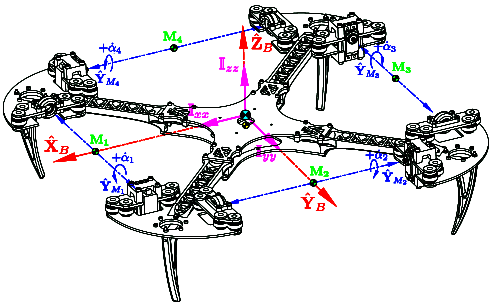
\includegraphics[width=0.9\textwidth]{figs/inertia-frame}
\caption{Inertial, mass and motor modules respective centers}
\label{fig:inertia-frame}
\end{figure}
\par
Each module's rotational center ($\vec{\mathbf{M}}_i=[\pm 195.16~~0~~0]$ or $[0~~\pm 195.16~~0]$ recalling Fig:\ref{fig:body-frame}) are spaced equally relative to the origin of motion, $\vec{\mathbf{O}}_b$, with a parallel axis arm $L_{arm}=195.16~~[\text{mm}]$ (highlighted in Fig:\ref{fig:inertia-frame}). To avoid notational confusion the term $\vec{L}_i$ is used to represent the vector displacement between the origin $\vec{\mathbf{O}}_b$ and each motor modules center of rotation $\vec{\mathbf{M}}_i$. The net inertial equation $J_b$, about the origin $\vec{\mathbf{O}}_b$ and dependent on the actuator position matrix $u\in\mathbb{U}$, can be calculated as:
\begin{subequations}
\label{eq:body-inertia}
\begin{equation}\label{eq:body-inertia.a}
\underset{\vec{\mathbf{O}}_b}{J_b(u)}=J_{body}+\sum_{i=1}^{4}J'_{\vec{\mathbf{M}}_i}~~~~[\text{kg.m}^2],~u\in\mathbb{U}
\end{equation}
Where $J'_{\vec{\mathbf{M}}_i}$ is the motor module inertia from Eq:\ref{eq:module-inertia} transformed to the origin $\vec{\mathbf{O}}_b$ using a parallel axis transformation with $m_{module}=190~[\text{g}]$:
\begin{equation}\label{eq:body-inertia.b}
J'_{\vec{\mathbf{M}}_i}=J_{\vec{\mathbf{M}}_i}+m_{module}\big(\vec{L}_i \cdot \vec{L}_i - \vec{L}_i\otimes\vec{L}_i\big)
\end{equation}
\end{subequations}
Although Eq:\ref{eq:body-inertia} does indeed produce the entire body's inertia, each equation to calculate $J_{\vec{\mathbf{M}}_i}$ involves cascaded transformations which may deteriorate the resultants certainty. Each motor module's inertia is first transformed to its respective centers of rotation from the center of masses, rotated as per the two servos and then finally transformed again to the body frame's origin. Alternatively transforming the inertial matrices about each sub-body's center of mass directly to the body frame origin will improve the reliability and generality of the produced inertial equations. It is also perhaps more intuitive to consider each sub-body's contribution individually, despite having been derived as combined inertial systems in the above equations. 
\begin{equation}\label{eq:body-net}
\underset{\vec{\mathbf{O}}_b}{J_b(u)}=\underset{\vec{\mathbf{O}}_b}{J'_{body}}+\sum_{i=1}^{4} \underset{\vec{\mathbf{O}}_b}{J_{inner}}+\sum_{i=1}^{4} \underset{\vec{\mathbf{O}}_b}{J_{middle}}~~~~u\in\mathbb{U}
\end{equation}
Isolating each body and considering its inertia separately then starting the inner rings, each having an inertia $J_{inner}$ with respect to its center of mass measured relative to its center of rotation. The following is then fundamentally different from Eq:\ref{eq:inertia.inner}, calculating the inner ring's inertial contribution about the origin $\vec{\mathbf{O}}_b$. \begin{subequations}
\label{eq:body-net-inner}
With a mass $m_{inner}$ and center of mass $C.M_{inner}$ relative to the center of rotation $\vec{\mathbf{M}}_i$ respectively:
\begin{equation}\label{eq:body-net-inner.a}
m_{inner}=92~~[\text{g}]
\end{equation}
\vspace{-10pt}
\begin{equation}\label{eq:body-net-inner.b}
C.M_{inner}=\begin{bmatrix}
-1.44 & 0 & 5.81
\end{bmatrix}^T~~[\text{mm}]
\end{equation}
The inner ring's inertial matrix about its center of mass was found to be:
\begin{equation}\label{eq:body-net-inner.c}
\underset{C.M}{J_{inner}}=\begin{bmatrix}
496.56 & -31.74 & 6.56\\
-31.74 & 1800.07 & 0.00\\
6.56 & 0 & 2048.98
\end{bmatrix}~~[\text{g.cm}^2]
\end{equation}
The inner ring's center of mass, rotated by $\lambda_i$ and $\alpha_i$ servos about their respective axes, is then:
\begin{equation}\label{eq:body-net-inner.d}
C.M'_{inner}=R_zR_y(\alpha_i)R_x(\lambda_i) \big(C.M_{inner}\big)
\end{equation}
So transforming the inertia from Eq:\ref{eq:body-net-inner.c}, still about the center of mass $C.M_{inner}$, but with axes aligned parallel with the body frame or $||\vec{\mathbf{O}}_b$:
\begin{equation}\label{eq:body-net-inner.e}
\underset{||\vec{\mathbf{O}}_b}{J'_{inner}(\lambda_i,\alpha_i)}=R_zR_y(\alpha_i)R_x(\lambda_i)\big(J_{inner}\big)R^{-1}_x(\lambda_i)R^{-1}_y(\alpha_i)\mathbb{R}^{-1}_z
\end{equation}
The direct difference from the new, rotated center of mass to the body origin $\vec{\mathbf{O}}_b$ is given by:
\begin{equation}
\Delta L = \vec{L}_i-C.M'_{inner}
\end{equation}
Then using the above in the parallel axis transformation theorem, adapted from Eq:\ref{eq:inertia.body.b}, to translate the rotated inertia $J'_{inner}$ to the center of the body frame $\vec{\mathbf{O}}_b$:
\begin{equation}
\underset{\vec{\mathbf{O}}_b}{J_{inner}}=\underset{||\vec{\mathbf{O}}_b}{J'_{inner}}+ m_{inner} \big((\Delta L \cdot \Delta L)\mathbb{I}_{3\times 3} - \Delta L \otimes \Delta L \big)
\end{equation}
\end{subequations}
Similarly, the same process for the middle rings rotated and translated inertia. For body with a mass and center of mass relative to the center of rotation respectively:
\begin{subequations}
\label{eq:body-net-middle}
\begin{equation}
m_{middle}=98~~[\text{g}]
\end{equation}
\vspace{-10pt}
\begin{equation}
C.M_{middle}=\begin{bmatrix}
-47.00 & 3.74 & -3.63
\end{bmatrix}^T~~[\text{mm}]
\end{equation}
The inertial matrix of the middle ring body, excluding the inner ring, about its center of gravity is:
\begin{equation}
\underset{C.M}{J_{middle}}=\begin{bmatrix}
2879.06 & 172.29 & 223.58\\
172.29 & 6268.97 & 13.33\\
223.58 & 13.33 & 8947.52\\
\end{bmatrix}~~[\text{g.cm}^2]
\end{equation}
The center of mass is rotated only by the $\alpha_i$ servo about the $\hat{Y}_{M_i'}$ axis:
\begin{equation}\label{eq:body-net-middle.d}
C.M'_{middle}=R_{z}R_{y}(\alpha_i)\big(C.M_{middle}\big)
\end{equation}
Then the rotated inertial matrix, aligned with axes parallel to the body frame origin $\vec{\mathbf{O}}_b$, follows:
\begin{equation}
\underset{||\vec{\mathbf{O}}_b}{J_{middle}}=R_zR_y(\alpha_i)\big(J_{middle}\big)R^{-1}_y(\alpha_i)R^{-1}_z
\end{equation}
The vector difference from the rotated center of mass to the body frame origin is calculated:
\begin{equation}
\Delta L = \vec{L}_i-{C.M'_{middle}}
\end{equation}
Which then leads to the parallel axis transformation of the middle ring's inertia to the body frame origin:
\begin{equation}
\underset{\vec{\mathbf{O}}_b}{J_{middle}}=\underset{||\vec{\mathbf{O}}_b}{J_{middle}}+m_{middle}\big((\Delta L\cdot\Delta L)\mathbb{I}_{3x3}-\Delta L \otimes \Delta L \big)
\end{equation}
\end{subequations}
Unless otherwise specified; any inertia $J_b(u)$ indicates an instantaneous calculated solution to Eq:\ref{eq:body-net} given a particular $u(t)\in\mathbb{U}$. The purpose of the derivations for rotated centers of mass in Eq:\ref{eq:body-net-inner} and Eq:\ref{eq:body-net-middle} is twofold; highlighting both the inertial contributions and the variable center of masses for each sub-body. As the origin of motion in the body frame $\mathcal{F}^b$ and the net body's center of mass are not coincidental, it is important to quantify the equation for the center of mass position, dependent on actuator positions $u\in\mathbb{U}$. In the general case for a collection of $n$ bodies, with each body's center of mass at some position $\vec{X}_i$ and each having a mass $m_i$, resultant center of mass is:
\begin{subequations}
\label{eq:mass-center}
\begin{equation}\label{eq:mass-center.a}
C.M = \frac{\sum_{i=1}^{n} m_i.\vec{X}_i}{\sum_{i=1}^{n} m_i}
\end{equation}
Using $\vec{X}_{inner}$ and $\vec{X}_{middle}$ as rotated centers of mass defined in Eq:\ref{eq:body-net-inner.d} and Eq:\ref{eq:body-net-middle.d} respectively, the entire assembly has a variable center of mass:
\begin{equation}\label{eq:mass-center.b}
C.M(u)=\frac{m_{body}.\vec{X}_{body}+\sum_{i=1}^{4} m_{inner}.\vec{X}_{inner}+\sum_{i=1}{4} m_{middle}.\vec{X}_{middle}}{m_{body}+\sum_{i=1}^{4} m_{inner} + \sum_{i=1}^{4} m_{middle}}
\end{equation}
Using a gravity vector $\vec{G}_b=R_I^b\vec{F}_g=R_I^b\begin{bmatrix}0&0&-9.81m\end{bmatrix}^T~[\text{N}]$, the resultant gravitational torque about the origin $\vec{\mathbf{O}}_b$ in the body frame $\mathcal{F}^b$ is:
\begin{equation}
\Delta C.G = \vec{\mathbf{O}}_b-C.M(u)
\end{equation}
\vspace{-15pt}
\begin{equation}\label{eq:grav-torque}
\vec{\tau}_g=\Delta C.G\times\vec{G}_b~~~~[\text{N.m}],\tau_g\in\mathcal{F}^b
\end{equation}
\end{subequations}
The net mass for the whole assembly is $1574.7~[\text{g}]$. For reference, the center of gravity when all actuators are at their zero positions is: $C.M=[0~0~-4.94]^T~[\text{mm}]$. Then, according to Eq:\ref{eq:body-net}, the inertial tensor for the net assembly at the rest conditions, $u=\vec{0}$, about the origin $\vec{\mathbf{O}}_b$ is:
\begin{equation}
J_b(\vec{0})=\begin{bmatrix}
317321.25 & 0 & 0\\
0 & 317321.25 & 0\\
0 & 0 & 628035.81
\end{bmatrix}
~~[\text{g.cm}^2]
\end{equation}
\newpage
%====================================================
\section{Electronics}
\label{sec:proto.layout}
%====================================================
{\centering
\fbox{
\begin{minipage}{\textwidth}
\centering
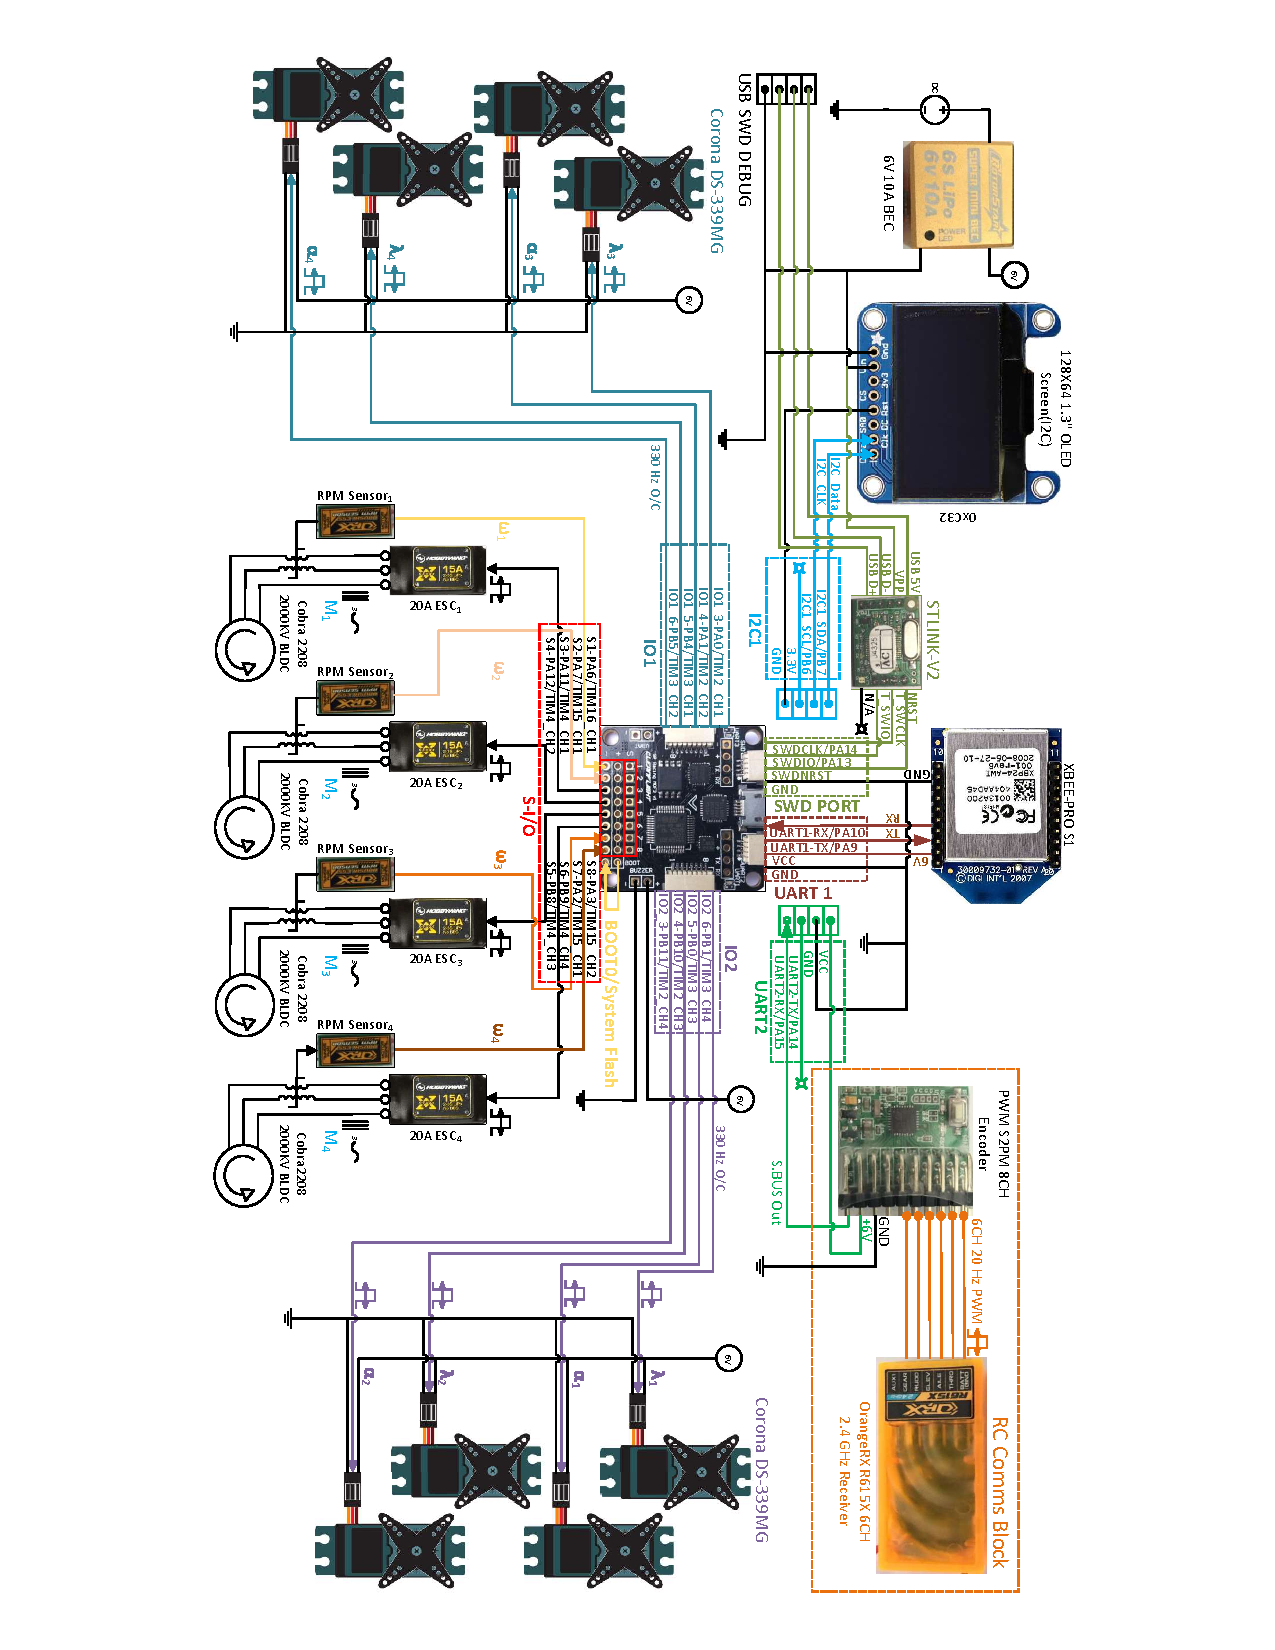
\includegraphics[width=0.95\textwidth]{pdfpages/electrical-schematic.pdf}
\end{minipage}
}
\captionof{figure}{Hardware schematic diagram}
\label{fig:electrical-schematic}
}
%-----------------------------------------------------
\newpage
%-----------------------------------------------------
An abstracted hardware diagram for the (electronic) system layout is shown in Fig:\ref{fig:electrical-schematic}. It's an illustration for the connection of different electronic peripherals used to aid the on-board control system. The structure of the implemented autopilot system and control loops are addressed later in Chapter:\ref{ch:flight}. This section aims to provide a brief overview of the specific modules used, their purpose and a description of how they're interfaced. No code structure or control loops are considered yet\ldots
\par
\begin{figure}[htbp]
\begin{subfigure}{0.5\textwidth}
\centering
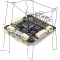
\includegraphics[width=0.9\textwidth]{figs/f3-deluxe}
\caption{SPRacing F3 deluxe flight controller}
\end{subfigure}
\begin{subfigure}{0.5\textwidth}
\centering
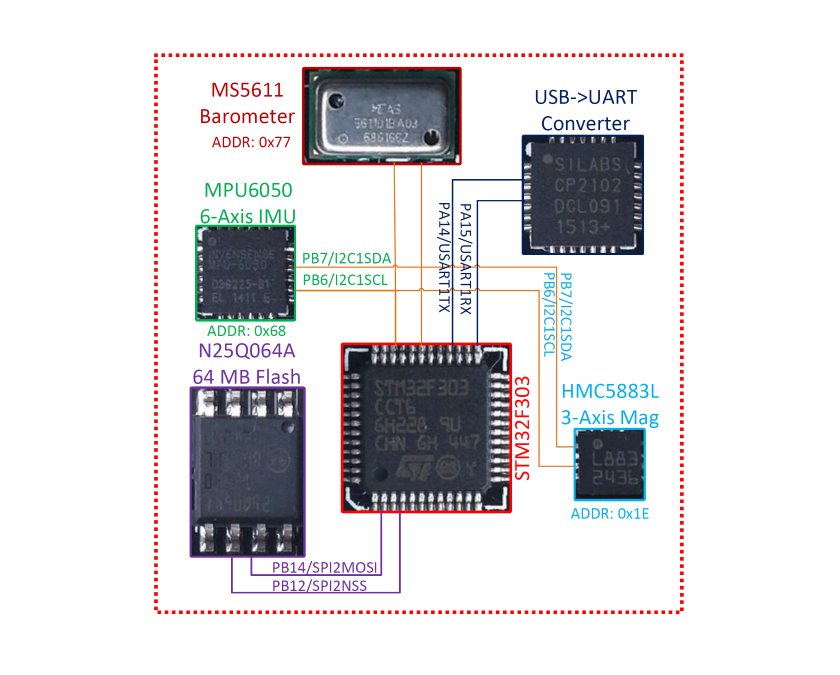
\includegraphics[width=0.9\textwidth]{figs/f3-deluxe-board}
\caption{F3 Deluxe on-board connections}
\label{fig:f3-deluxe-board}
\end{subfigure}
\caption{SPRacing F3 deluxe layout}
\label{fig:f3-deluxe-layout}
\vspace{-10pt}
\end{figure}
The embedded system is constructed around an ARM STM32F303\cite{stm32f303} based $\mu$C. The micro-processor board is a commercial flight control board, specifically an SPRacing F3 Deluxe\cite{spracing}\footnote{CleanFlight or BetaFlight opensource software is regularly used for the F3 but its hardware specifications are not openly avaiable. The reverse engineered electrical schematic for the board is included in Appendix:\ref{app:deluxe-diagram}}, which has had its bootloader removed and custom firmware, unique to this project, developed for it. That software is later described in Chapter:\ref{ch:flight}; the I/O for all the peripherals are however detailed here. The flight-controller has the following onboard peripherls: an I2C MPU-6050\cite{mpu6050} 6-axis gyroscope \& accelerometer with an I2C connected HMC5883\cite{hmc5883} magnetometer compass, an I2C MS5611\cite{ms5611} barometer and finally 64 Mb of SPI flash memory. The electrical schematic diagram of those peripherals and the core STM32F303 microprocessor is detailed in Appendix:\ref{app:deluxe-diagram} but their connection(s) and layout are shown in Fig:\ref{fig:f3-deluxe-layout}. 
\par
\begin{minipage}{\textwidth}
\par
\begin{wrapfigure}{r}{0.49\textwidth}
\vspace{3pt}
\centering
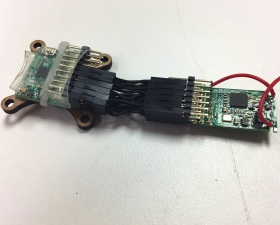
\includegraphics[width=0.49\textwidth]{figs/ppm-sbus}
\caption{SBUS converter \& 6CH receiver}
\label{fig:ppm-sbus}
\end{wrapfigure}
\par
\emph{\color{Gray}\\ The combination of above sensors fused for state estimation and their associated filtration algorithms are dealt with in Section:\ref{sec:simulation.state} of Chapter:\ref{ch:simulation}.\\}
\par
Two separate wireless communication peripherals are used. First the system relays full state information, for a complete 6-DOF autopilot system, from a ground control station using 2.4 GHz XBEE S1 module(s)\cite{xbees1}, connected via USART. Secondly, an augmented pilot control input system, fail safe and secondary to the autopilot loop, is transmitted through 6 Channel 2.4 GHz R/F comms. The 6 CH received signals, otherwise permeated as six individual 20 KHz PWM signals via an OrangeRx R615x\cite{r615x} receiver, are encoded into a single proprietary S.BUS data stream (Fig:\ref{fig:ppm-sbus}). 
\end{minipage}
\par
The need for an S.BUS encoder\cite{sbusencoder} comes about as a consequence of the introduction of the 8 additional servos. As a result, there are no longer 6 free additional timer I/O channels which can be dedicated to input capture of those RC channels. 
\par
Encoding the received data to a serial communication protocol means the 6CH data can be processed on a single serial RX line. The S.Bus encoder implements a USART derivative communications standard, Fig:\ref{fig:sbus} shows the sampled data stream used to ascertain the standard's following parameters:
\par
\begin{tabularx}{\textwidth}{X X}
\begin{minipage}{\textwidth}
\begin{itemize}[itemsep=0em]
\item 25 Bytes per packet
\item 8-Bit byte length
\item 1 Start byte 0x240
\item 1 Byte of flags
\item 1 Stop byte 0x0
\item Bytes are:
\vspace{-5pt}
\begin{itemize}[itemsep=0em]
\item MSB First
\item 1 start \& 2 stop bits
\item Even parity bit
\item Inverted
\item 100000 baud (b.s$^{-1}$)
\end{itemize}
\vspace{-5pt}
\end{itemize}
\end{minipage}
&
\begin{minipage}{\textwidth}
\begin{itemize}[itemsep=0em]
\item 22 bytes of CH data 
\item Each channel's data is 11 bits long
\item 16CH encoded
\item Channel data is little endian prioritized
\item 14 ms idle time between packets
\item Packets are arranged:
\end{itemize}
{
$\overbrace{[0x240]}^{Start~byte}\overbrace{[8B_1][3B_2}^{CH1}|\overbrace{5B_2][6B_3}^{CH2}|\overbrace{2B_3][8B_4][1B_5}^{CH3}|\ldots$
\\
$\overbrace{7B_5][4B_6|}^{CH4}~\longrightarrow~\overbrace{3B_22][8B_23]}^{CH16}\overbrace{[8B_24]}^{Flags}\overbrace{[0x00]}^{Stop~byte}$
}
\end{minipage}
\\
\end{tabularx}
\begin{figure}[hbtp]
\centering
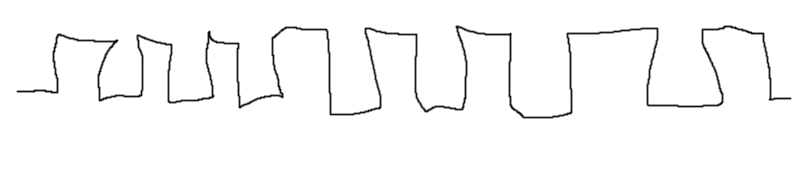
\includegraphics[width=\textwidth]{figs/sbus}
\caption{S.BUS data stream}
\label{fig:sbus}
\vspace{-10pt}
\end{figure}
\par
{\color{red}
The received information from the transmitted 6 channels is filtered through a moving average IIR$^\dagger$ filter. The filters difference equation is as follows: 
\begin{equation}
y_n = \big(1-\frac{1}{N}\big)y_{n-1}+\frac{1}{N}x_n
\end{equation}
Moving over an average of $N=5$ samples. The signal's sample rate is sufficiently fast enough such that the digital filter's frequency response isn't of consequence. Similarly all the measured RPM signals are filtered as well. Any received signals referred to are all post filtration. Filtering for non-IMU state estimates is separately performed on the Ground Control Station computer.}
\par
Each of the eight digital servo actuators are driven individually from 330 Hz center aligned PWM timer output compare channels (TIM2:CH1$\rightarrow$CH4 \& TIM3:CH1$\rightarrow$CH4). Center alignmed PWM\footnote{Unqiue to the STM32 \& PIC micros, supported by the ARM mthumb instruction set.} reduces current spikes at the start of each timing cycle. Output pulses typically range from 1ms - 2ms to linearly control the rotational position. The exact range and transfer function is empirically determined next in Subsection:\ref{subsec:proto.design.transfer}. The four 20A brushless DC speed controllers (ESCs) are each driven from a 20 Hz PWM output (TIM4:CH1$\rightarrow$CH4), similarly with 1ms - 2ms input pulse widths. There are a total of 12 PWM output compare signals drawn from the $\mu$C. Servos are powered by a regulated 6V DC 10A power supply \cite{rotorstar} whilst the ESCs switch unregulated 14.1 V DC from an externally tethered power supply. The DC supply could potentially be drawn from an on-board battery bank but that would add significant weight to an already heavy platform.
\par
There's no integrated feedback for instantaneous RPM values from the ESCs. Using discrete OrangeRX BLDC RPM sensors \cite{orangerpm}, that measure switching phases across two of the three motor phases, the exact RPM can be ascertained.
\par
\begin{figure}[htbp]
\begin{subfigure}{0.5\textwidth}
\centering
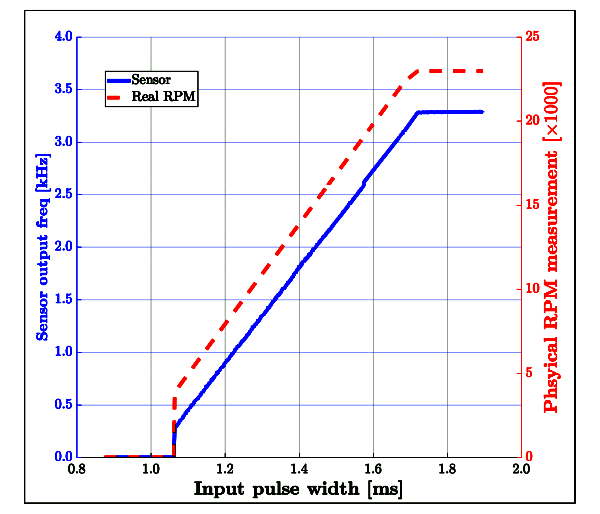
\includegraphics[width=\textwidth]{graphs/rpm-sensor-noload}
\caption{RPM sensor plot - no load}
\label{fig:rpm-sensor-noload}
\end{subfigure}
\begin{subfigure}{0.5\textwidth}
\centering
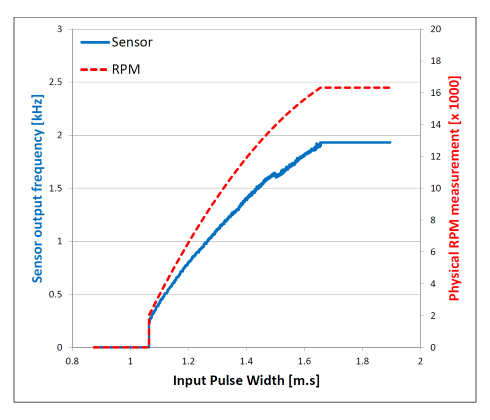
\includegraphics[width=\textwidth]{graphs/rpm-sensor-prop}
\caption{RPM sensor plot - 6X4.5 prop}
\label{fig:rpm-sensor-prop}
\end{subfigure}
\caption{RPM sensor calibration plots}
\label{fig:rpm-sensor}
\end{figure}
The switching signal of a 3-Phase induction motor\footnote{Although termed DC motors, BLDC motors are actually 3-$\phi$ IM motors which, combined with an ESC, behave like closed loop DC motors.} is\cite{vfd}:
\begin{equation}
F_{rps}=\frac{2\times F_{poles}}{\text{No. of rotor poles}}~~[Hz]
\end{equation}
The signal produced by the RPM sensors varies the period of a 50\% duty cycle square wave, the wave frequency is directly proportional to that of the pole's switching frequency. The RPM sensor's output signal is then calibrated to a gain of 7 for the 14 pole BLDC Cobra motors used. That gain is verified with the linear relationship(s) is shown in Fig:\ref{fig:rpm-sensor}. Knowing exact RPM rates means the subsequent thrust and aerodynamic torques for the control plant inputs can be calculated.
\par
\begin{figure}[hbtp]
\begin{subfigure}{0.5\textwidth}
\centering
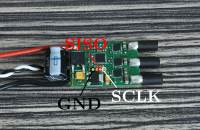
\includegraphics[width=0.98\textwidth]{figs/xrotor-20A}
\caption{XRotor 20A ESC connection guide\cite{xrotor}}
\label{fig:xrotor-20A}
\end{subfigure}
\begin{subfigure}{0.5\textwidth}
\centering
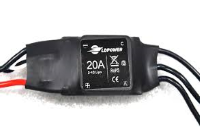
\includegraphics[width=0.98\textwidth]{figs/ldpower-20A}
\caption{LDPower 20A ESC with RPM sensor}
\label{fig:ldpower-20A}
\end{subfigure}
\caption{BLDC electronic speed controllers}
\end{figure}
The speed controllers, although LDPower 20A devices, are all re-flashed with BLHeli\footnote{LDPower 20A ESCs(Fig:\ref{fig:ldpower-20A}) match Hobbywing Xrotor 20A speed controllers (Fig:\ref{fig:xrotor-20A}), they both use SiLabs F396 MCUs. Physical rotational values in the plots Fig:\ref{fig:rpm-sensor} were measured with optical encoders.}\cite{BLHeli} firmware. The custom software on the ESC's $\mu$C can provide greater refinement over parameter configuration like the deflection range of inputs, however, default values were used. The plot in Fig:\ref{fig:rpm-sensor-noload} shows the linear RPS (in Hz) speed curve for an unloaded motor; similarly in Fig:\ref{fig:rpm-sensor-prop} shows the speed curve when loaded for a 6-inch prop. 
\par
It's interesting to note that the loaded speed curve is slightly parabolic (Fig:\ref{fig:rpm-sensor-prop}), resulting from the aerodynamic drag term which is quadratic with respect to rotational velocity, expanded on in Sec:\ref{subsec:dynamics.aero.bem}. Moreover, when the motor is torque loaded by the propeller, the ESC current limits rotational speeds at just over 16 000 RPM. The sensor feedback is used for minor loop RPM control.
\par
Timers channels are used to measure the varying frequency output from the RPM sensors. General purpose Timers 15 (TIM15:CH1$\rightarrow$CH2), 16 (TIM16:CH1) and 17 (TIM17:CH1) are configured to capture the input PWM signal generated by the speed sensors. Included on the I2C communciation line is an I2C O-LED display for debugging and status update purposes.
\par
Any STM32 $\mu$controller is programmed through a dedicated debugging device. The ST-Link V2\cite{st-link} is the current proprietary device which, itself, is a specially programmed STM32F10 chip. The chip connects to the dedicated \textbf{S}erial \textbf{W}ire \textbf{D}ebugging ports of the target STM (\emph{SWD-CLK, SWD-IO} \& \emph{SWD-NRST}) and is interfaced via regular USBD+ and USBD- data lines. 
%====================================================
\subsection{Actuator Transfer Functions}
\label{subsec:proto.design.transfer}
%====================================================
\subsubsection*{Servo Transfer Functions}
%====================================================
\begin{figure}[htbp]
\centering
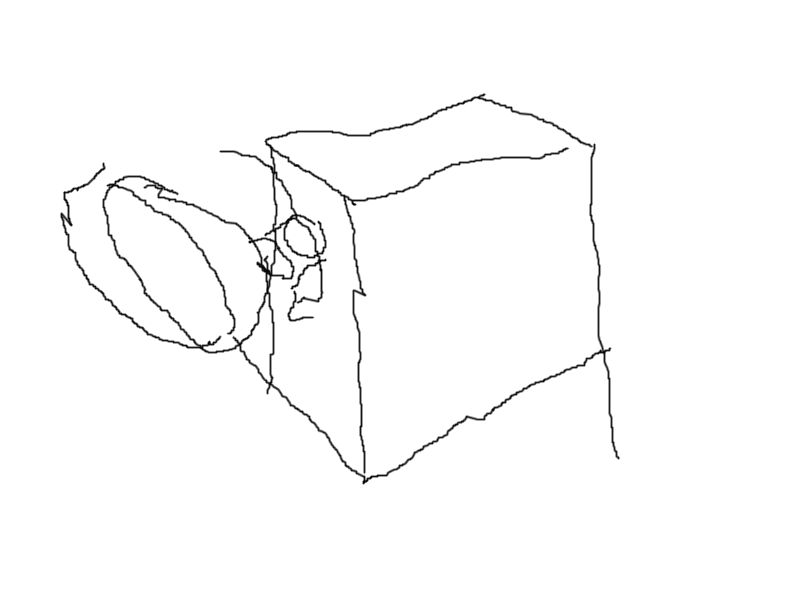
\includegraphics[width=0.7\textwidth]{figs/servo-position}
\caption{Servo transfer function test rig}
\label{fig:servo-position}
\end{figure}
The full scale deflection of each digital servo is in fact greater than its quoted 180\textdegree ~range. Each servo has a rotational range of around 230\textdegree ~(Fig:\ref{fig:servo-range}). The exact characteristics for every servo differ slightly and thus individual transfer functions for each of the 8 servos are used in simulation. In the prototype control loop the servos are left in open loop; the major loop controller coefficients are expected to account for minor loop actuator dynamics. With that being said, for such an expectation to be validated the simulation would need to accurately represent the servo's response. 
\par
Seeing that the 180\textdegree ~limitation was imposed as a design decision; one of the first points of contention is the effect such a constraint would have on the feasible operating trajectories. The control algorithms derived in Chapter:\ref{ch:control} are first tested with an ideal, continuous rotation servo actuator with similar rate limits and transfer characteristics. Later the servo saturation limitations are introduced and the constraints to feasibly achievable trajectories are investigated.
\begin{figure}[htbp]
\centering
\begin{subfigure}{0.49\textwidth}
\centering
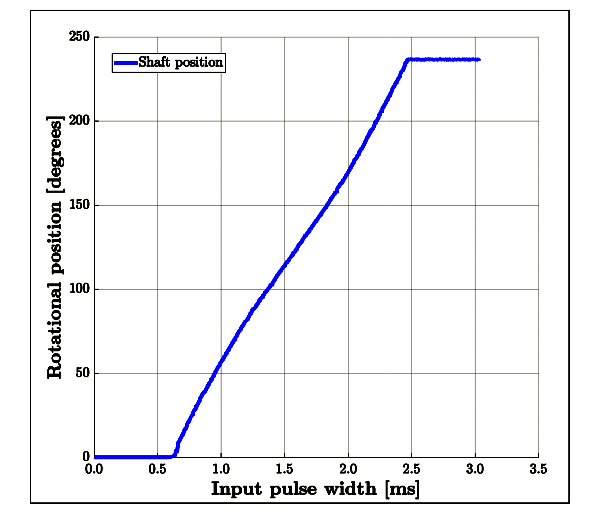
\includegraphics[width=\textwidth]{graphs/servo-range}
\caption{DS339-MG full Range}
\label{fig:servo-range}
\end{subfigure}
\begin{subfigure}{0.49\textwidth}
\centering
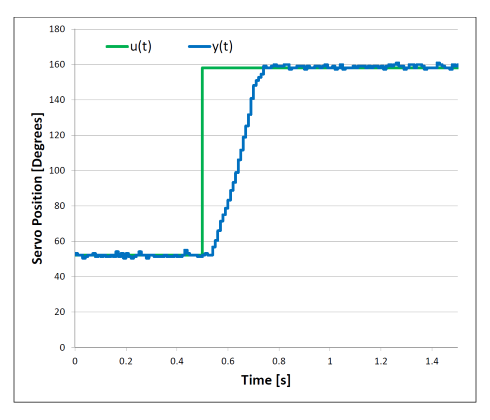
\includegraphics[width=\textwidth]{graphs/servo-step}
\caption{DS339-MG Step Response}
\label{fig:servo-step}
\end{subfigure}
\caption{Unloaded servo transfer characteristics}
\label{fig:servo-no-load}
\vspace{-10pt}
\end{figure}
\par
For the servo \footnote{Servo number 1 of 8 tested, $\lambda_1$, is used for transfer function demonstration. For simulation, each of the 8 servos were individually determined.} whose rotational range and step response are shown in Fig:\ref{fig:servo-no-load}, the relationship between the input pulse-width $x~[m.s]$ and the rotational output position $y~degrees$ is given by:
\begin{equation}\label{eq:servo-range}
y(x)=
\begin{cases}\begin{array}{ll}
0\text{\textdegree} & ~~x<0.65~m.s\\
129.12x-82.64 & ~~0.64~m.s \leq x \leq 2.46~m.s\\
230\text{\textdegree} & ~~x>2.46~m.s\\
\end{array}
\end{cases}
\end{equation}\par
\begin{figure}[hbtp]
\vspace{-20pt}
\centering
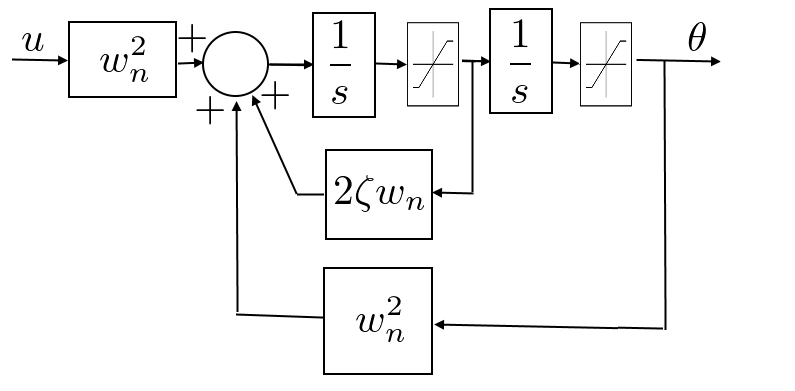
\includegraphics[width=0.8\textwidth]{figs/servo-block}
\caption{Servo block diagram}
\label{fig:servo-block}
\end{figure}
Although, in practice, the equation Eq:\ref{eq:servo-range} is changed such that 0\textdegree ~offset is taken at around a 50\% input, making its operational range $\pm 90$\textdegree . Each servo is mechanically rate limited to $60\text{\textdegree}/0.15s$ or $400~RPS$ with a dead time of $\approx 1.2~m.s$ and a mechanical deadband of $\leq4\mu s$. The net transfer block for the servo is shown in Fig:\ref{fig:servo-block}, including non-linearities but neglecting the deadband. Each servo has an approximate (\emph{critically damped}) second order transfer function$^{\dagger}$:
\begin{subequations}\label{eq:servo-transfer}
\begin{equation}
G_{servo}(s)=e^{-t_d s}\frac{w_n^2}{s^2+2\zeta w_n s + w_n^2}
=e^{-0.012s}\frac{(15.717)^2}{s^2+2(1)(15.717)+(15.717)^2}
\end{equation}
With saturation limits:
\begin{equation}
Y_{servo}(s)=
\begin{cases}\begin{array}{ll}
0\text{\textdegree} & ~~|U(s)|<0.65\\
G(s) & 0.65 \leq |U(s)| \leq 2.46\\
230\text{\textdegree} & ~~|U(s)|>2.46\\
\end{array}
\end{cases}
\end{equation}
\end{subequations}
The transfer plot in Fig:\ref{fig:servo-step} is that of an unloaded servo's response. When loaded with the inner ring assembly (Fig:\ref{fig:servo-inner-character}) the plant response {\color{Blue}$\mathbf{y(t)}$} is consistent with that of Eq:\ref{eq:servo-transfer}. Despite rotating a load mass and hence requiring a greater torque, the servo's characteristics remains unchanged, even when the BLDC motor (with a 6$\times$4.5" prop) is spun an average rate of 6500 RPM, {\color{Red}$\mathbf{y'(t)}$}, further tensioning the assembly.
\begin{figure}[hbtp]
\begin{subfigure}{0.5\textwidth}
\centering
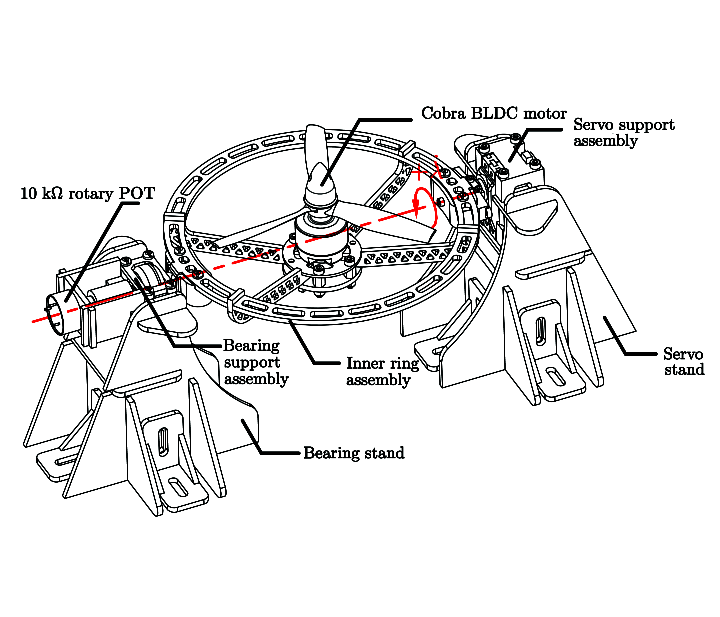
\includegraphics[width=0.98\textwidth]{figs/servo-inner}
\caption{Inner ring servo rig}
\label{fig:servo-inner}
\end{subfigure}
\begin{subfigure}{0.5\textwidth}
\centering
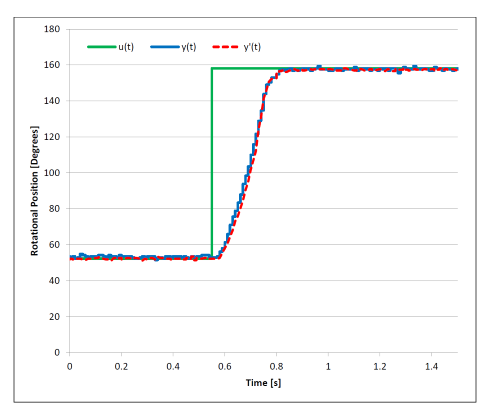
\includegraphics[width=0.98\textwidth]{graphs/servo-step-inner}
\caption{Servo response plot}
\label{fig:servo-step-inner}
\end{subfigure}
\caption{Inner ring servo characteristics}
\label{fig:servo-inner-character}
\vspace{-10pt}
\end{figure}
\par
However, in Fig:\ref{fig:servo-middle-character}, the response for a servo driving the middle ring is shown. Its rate transients remains the same but oscillations at the settling point are introduced by the larger mass being driven. These are product of the structure's flex within the middle ring assembly and \emph{not from the servo plant}. The rotational position was measured (Fig:\ref{fig:servo-middle}) with respect to the bearing supported output shaft, coaxial to the servos, and \emph{not} the servo's output shaft. The oscillations are still present under load, {\color{Red}$\mathbf{y'(t)}$}, despite the frame being further tensioned by a thrust vector. The mechanical harmonics can be accounted for by either introducing a more rigid sub-frame, limiting the maximum angular rate or applying a damping minor loop controller. The latter would require a \emph{virtual} closed loop with an approximated error rate as the prototype structure doesn't incorporate positional feedback for each motor module.
\begin{figure}[hbtp]
\begin{subfigure}{0.5\textwidth}
\centering
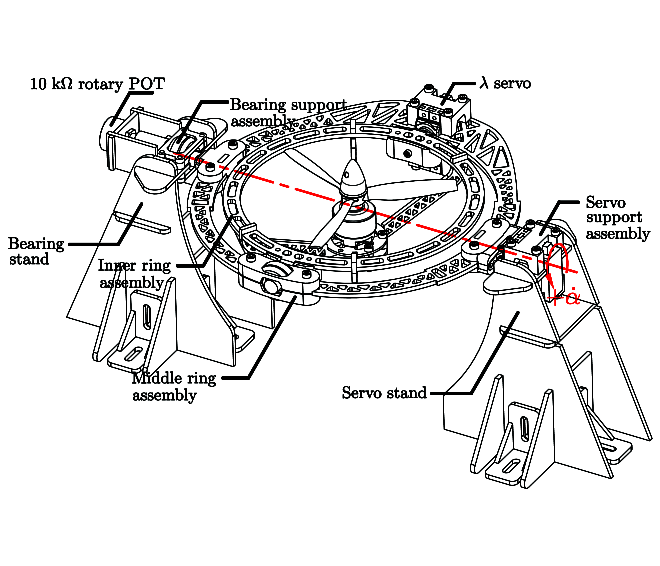
\includegraphics[width=0.98\textwidth]{figs/servo-middle}
\caption{Middle ring servo test rig}
\label{fig:servo-middle}
\end{subfigure}
\begin{subfigure}{0.5\textwidth}
\centering
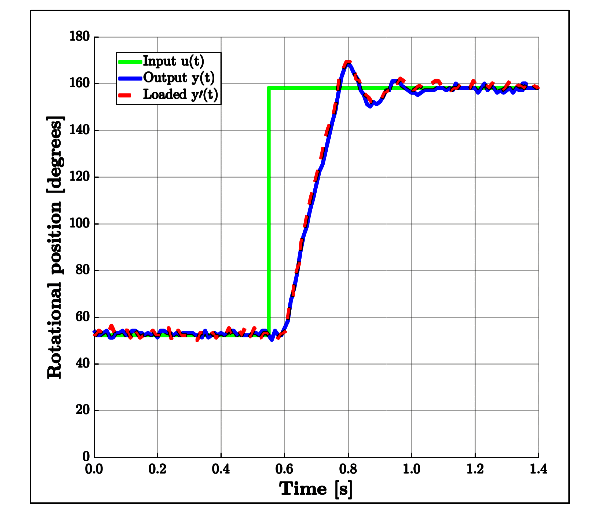
\includegraphics[width=0.98\textwidth]{graphs/servo-step-middle}
\caption{Servo response plot}
\label{fig:servo-step-middle}
\end{subfigure}
\caption{Middle ring servo characteristics}
\label{fig:servo-middle-character}
\vspace{-20pt}
\end{figure}
\subsubsection*{BLDC Transfer Functions}
Each Cobra 2208 BLDC motor, when loaded with a 6$\times$4.5 propeller has a quadratic speed curve, Fig:\ref{fig:bldc-range}. This is as a result of the propeller's opposing aerodynamic drag, \emph{appromixately} proportional to the square of the propellers angular velocity (Sec:\ref{subsec:dynamics.aero.bem}). 
\par
\begin{figure}[htb]
\vspace{-15pt}
\centering
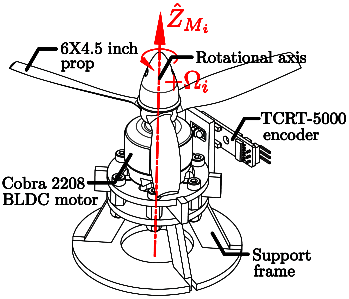
\includegraphics[width=0.44\textwidth]{figs/bldc-rpm}
\caption{BLDC rpm speed calibration and transfer function rig}
\label{fig:bldc-rpm}
\vspace{-15pt}
\end{figure}
The relationship\footnote{The input range can be adjusted in BLHeli ESC software to improve input resolution, but was left unchanged.} between input pulse-width to the ESCs and output RPM sensor signal (Fig:\ref{fig:bldc-range}) is:
\begin{equation}
y(x)=
\begin{cases}\begin{array}{ll}
0 & ~~x<1.065~m.s\\
-20593x^2 + 80187x - 60004 & ~~1.065~m.s \leq x \leq 1.655~m.s\\
16300\text{\textdegree} & ~~x>1.655~m.s\\
\end{array}
\end{cases}
\label{eq:bldc-range}
\end{equation}
\par
The upper limit in Eq:\ref{eq:bldc-range} and the motor's step response are both governed by the ESC's maximum current limit; in this case 20A. Imposing 10A current limiting (a consequence of using lower power ESCs), the plot for {\color{YellowGreen}$\mathbf{c(t)}$} in Fig:\ref{fig:bldc-step}, significantly restricts the motor's transient and steady-state performance. The motor's step response, {\color{Purple}$\mathbf{y(t)}$} has a negligible dead time and 2$^{nd}$ order dynamics\footnote{It can't be stressed enough how much the BLHeli ESC firmware improved dynamic response of the motors}, far faster than the servo's plant. The motors transfer function for speed in RPM is:
\begin{subequations}\label{eq:bldc-transfer}
\begin{equation}
G_{BLDC}(s)=\frac{1}{\big(1+1.7583s\times 10^{-3}\big)\big(1+1.7494s\times 10^{-3}\big)}
\end{equation}
And saturation limits:
\begin{equation}
Y_{BLDC}(s)=
\begin{cases}\begin{array}{ll}
0\text{\textdegree} & ~~|U(s)|<1.065\\
G(s) & 1.065 \leq |U(s)| \leq 1.655\\
16300 & ~~|U(s)|>1.655\\
\end{array}
\end{cases}
\end{equation}
\end{subequations}
\begin{figure}[hbtp]
\vspace{-20pt}
\begin{subfigure}{0.5\textwidth}
\centering
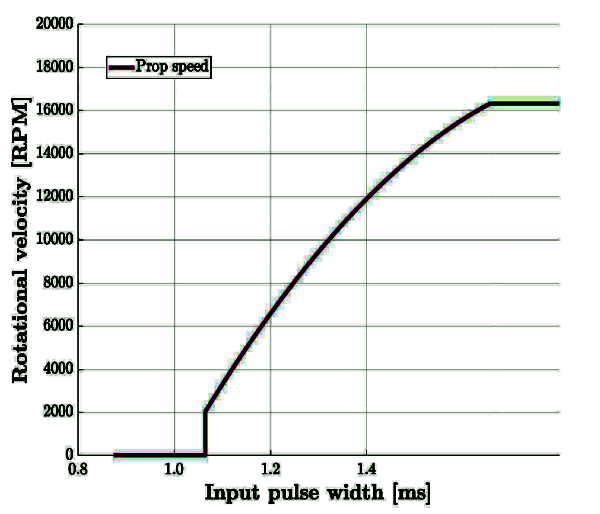
\includegraphics[width=0.98\textwidth]{graphs/bldc-range}
\caption{BLDC RPM range}
\label{fig:bldc-range}
\end{subfigure}
\begin{subfigure}{0.5\textwidth}
\centering
\includegraphics[width=0.98\textwidth]{graphs/BLDC-step}
\caption{Cobra BLDC step response}
\label{fig:bldc-step}
\end{subfigure}
\vspace{-10pt}
\caption{BLDC motor characteristics}
\vspace{-20pt}
\end{figure}
%====================================================
